\chapter{Literature review}

\section*{Introduction}
\subsection*{Methodology}
The approach adopted in this literature review is intermediate between a systematic approach and a survey of related works.
The justification for this singular approach is that many domains are presented, some containing several tens of thousands of articles.
For this reason, a systematic approach would be too cumbersome, while a survey would not reflect the richness of each field.

First, the scope of the literature review will be defined through research hypotheses.
Once these hypotheses are created, queries will be made on a bibliographic database.
The queries will be performed on Scopus~\footnote{https://www.scopus.com/}, which offers a larger number of references than the Web of Science and more tools for query design.

The results obtained will then be analyzed from several angles. First of all, the evolution of the volume of publications returned by the query, to attempt to represent the interest in the topic.
Secondly, an analysis of the keywords will be made through VOSviewer~\footnote{https://www.vosviewer.com/} "a software tool for constructing and visualizing bibliometric networks".
Especially VOSviewer allows to visualize bibliographic features such as the network of authors or of keywords.
The keywords used by the different articles fetched by the request provide valuable insights on the evolution of a given field, especially on its interdisciplinary aspect.
Finally, a review of some of the most influential articles from the query result will be discussed.
The influence criteria will be the number of citations.

This methodology aims to provide a sufficient understanding of the interest and evolution of the topics explored, as well as answers related to the subproblematics exposed.

\subsection*{Hypotheses}
This manuscript is limited in the scientific domain investigated.
Thus, the following working hypotheses will delimit the work presented.

\begin{itemize}
    \item 1. On social media data: social media data have a low ratio information/noise and are as trustworthy as phone calls. Clean, well-written textual data are then excluded.
    \item 2. On crisis management: the crisis management context is particular and this manuscript focuses on the response phase and its context.
    \item 3. On improving the decision making process: improving decision making means improving situational awareness and coordination among the various actors.
\end{itemize}

Having these hypotheses, the literature review presented in this chapter explores the context around the different problematics raised in the previous chapter.
As a reminder, the main problem of this manuscript is: \emph{How to design an information system able to automatically manage and deliver relevant information extracted from social media data during crisis response?}
This main problematic is decomposed among three sub problematics:

\begin{itemize}
    \item What information that can be obtained from social media is relevant to the decisiom makers in crisis response?
    \item How can these information be obtained, in the context of crisis informatic?
    \item How are these information organised to deliver the value expected by decision makers?
\end{itemize}

The first section of this chapter presents the work related to the main problematic and specially systems developped to automatically process social media during crisis response.
Then, the second section explores the first sub problematic and the different representations of information used by previous work.
Finally, the third section overlook social media processing by NLP in general to provide context for the second sub problematic.
As the last sub problematic is similar to the one of the main problematic, its literature review will be merge into the first section.

\section{Information systems for crisis response fed with social media data}
Chapter 1 identified the opportunities offered by social media to support crisis response.
Many researchers explored that opportunities and built systems and architecture to mine data and provide their insights to decision makers.
This first part of the literature review intends to highlight the systems built for this purpose.
The question that this parts aims to answer is: \emph{What are the existing social media processing system developped for crisis response over the years?}

To answer this question, the following request was made on the Scopus database.

\begin{itemize}
    \item SUBJAREA(comp)
    \item AND (TITLE-ABS-KEY({crisis management} or {crisis response} or contingency or {disaster response} or {disaster management}))
    \item AND (TITLE-ABS-KEY ({social media} or twitter))
    \item AND (TITLE-ABS-KEY(system and processing))
    \item AND ( EXCLUDE ( DOCTYPE,"re" ) OR EXCLUDE ( DOCTYPE,"cr" ) )
\end{itemize}

The request returns papers that:

\begin{itemize}
    \item Are in the computer science domain, as this domain contains both the AI and Information Systems domains.
    \item Are centered around crises|disasters management|response or contingency plans.
    \item That present systems that process data
    \item Papers that present conference tracks and reviews are excluded.
\end{itemize}

The request returns 96 documents, published between 2011 and 2021.
The beginning of this domain of research corresponds to the democratization of social media, with the development of social media plaforms happening during the 2000-2010 period (Figure~\ref{literature:crisis-informatic-hist}).
Naturally, the field has developed, driven by the need of crisis management organizations and the public interest benefit it promises.

\begin{figure}[htb]
    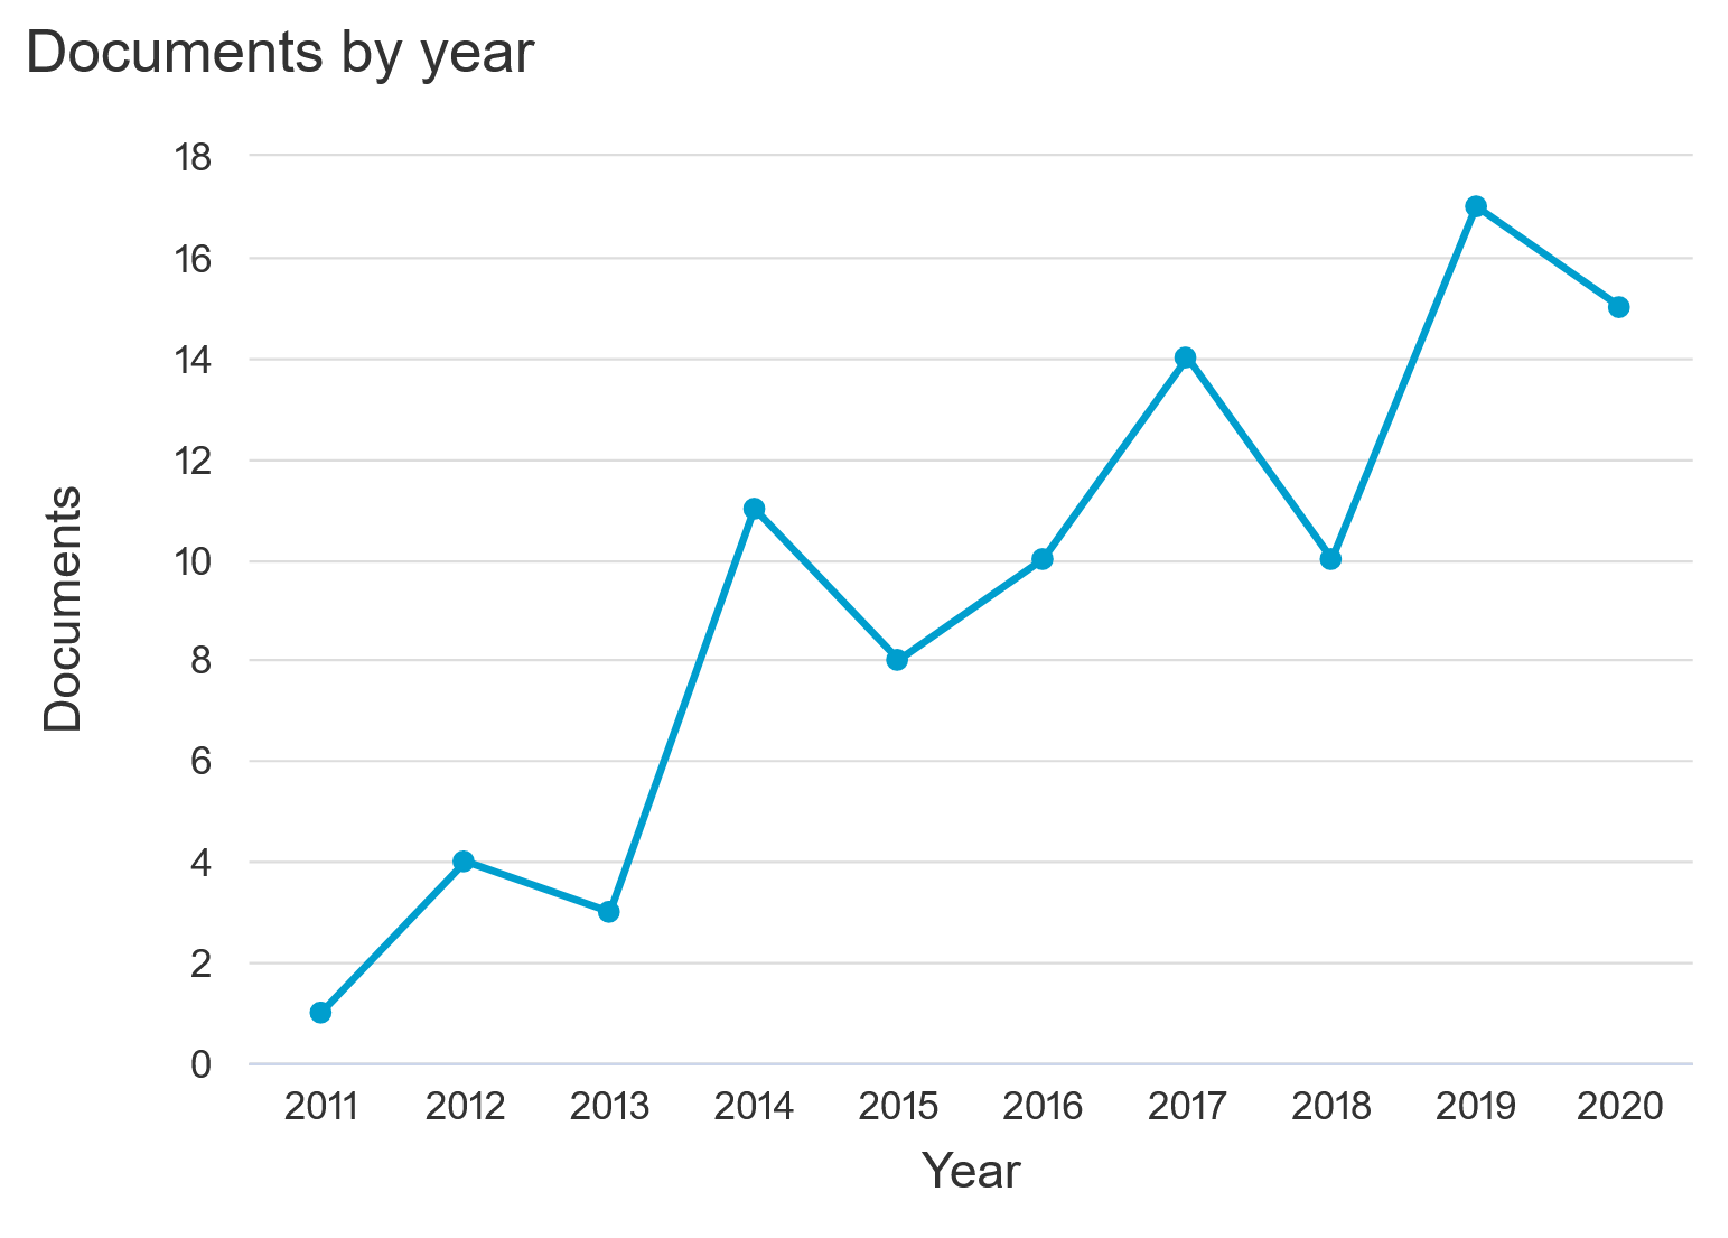
\includegraphics[width=\textwidth]{figures/chap-2/crisis-informatic-hist.pdf}
    \caption{Timelime of the volume of contributions per years for the crisis informatic domain. The year 2021 is excluded because the year is not complete at the time of writing.}
    \label{literature:crisis-informatic-hist}
\end{figure}

The network provided by VOSviewer (Figure~\ref{literature:crisis-informatic-overlay}) do not reveal any significant cluster of keywords, which is not surprising considering the youth of the domain.
However, the timeline of publication (represented by the color variation) provides interesting insight on the direction of the domain.
Years around 2016 were mostly focused on data analyses of the different datasets available.
Then, the following years saw the development of more and more automation.
Artificial intelligence, machine learning and natural language processing appeared in that chronological order, coinciding with the progress made in these areas.
More recently, deep learning models to process text and/or images are appearing, as well as new opportunities created by the internet of things and the development of the concept of smart cities.
It is also very interesting to observe that social sciences and computers sciences are completely blended altogether.

\begin{landscape}
    \begin{figure}[htb]
        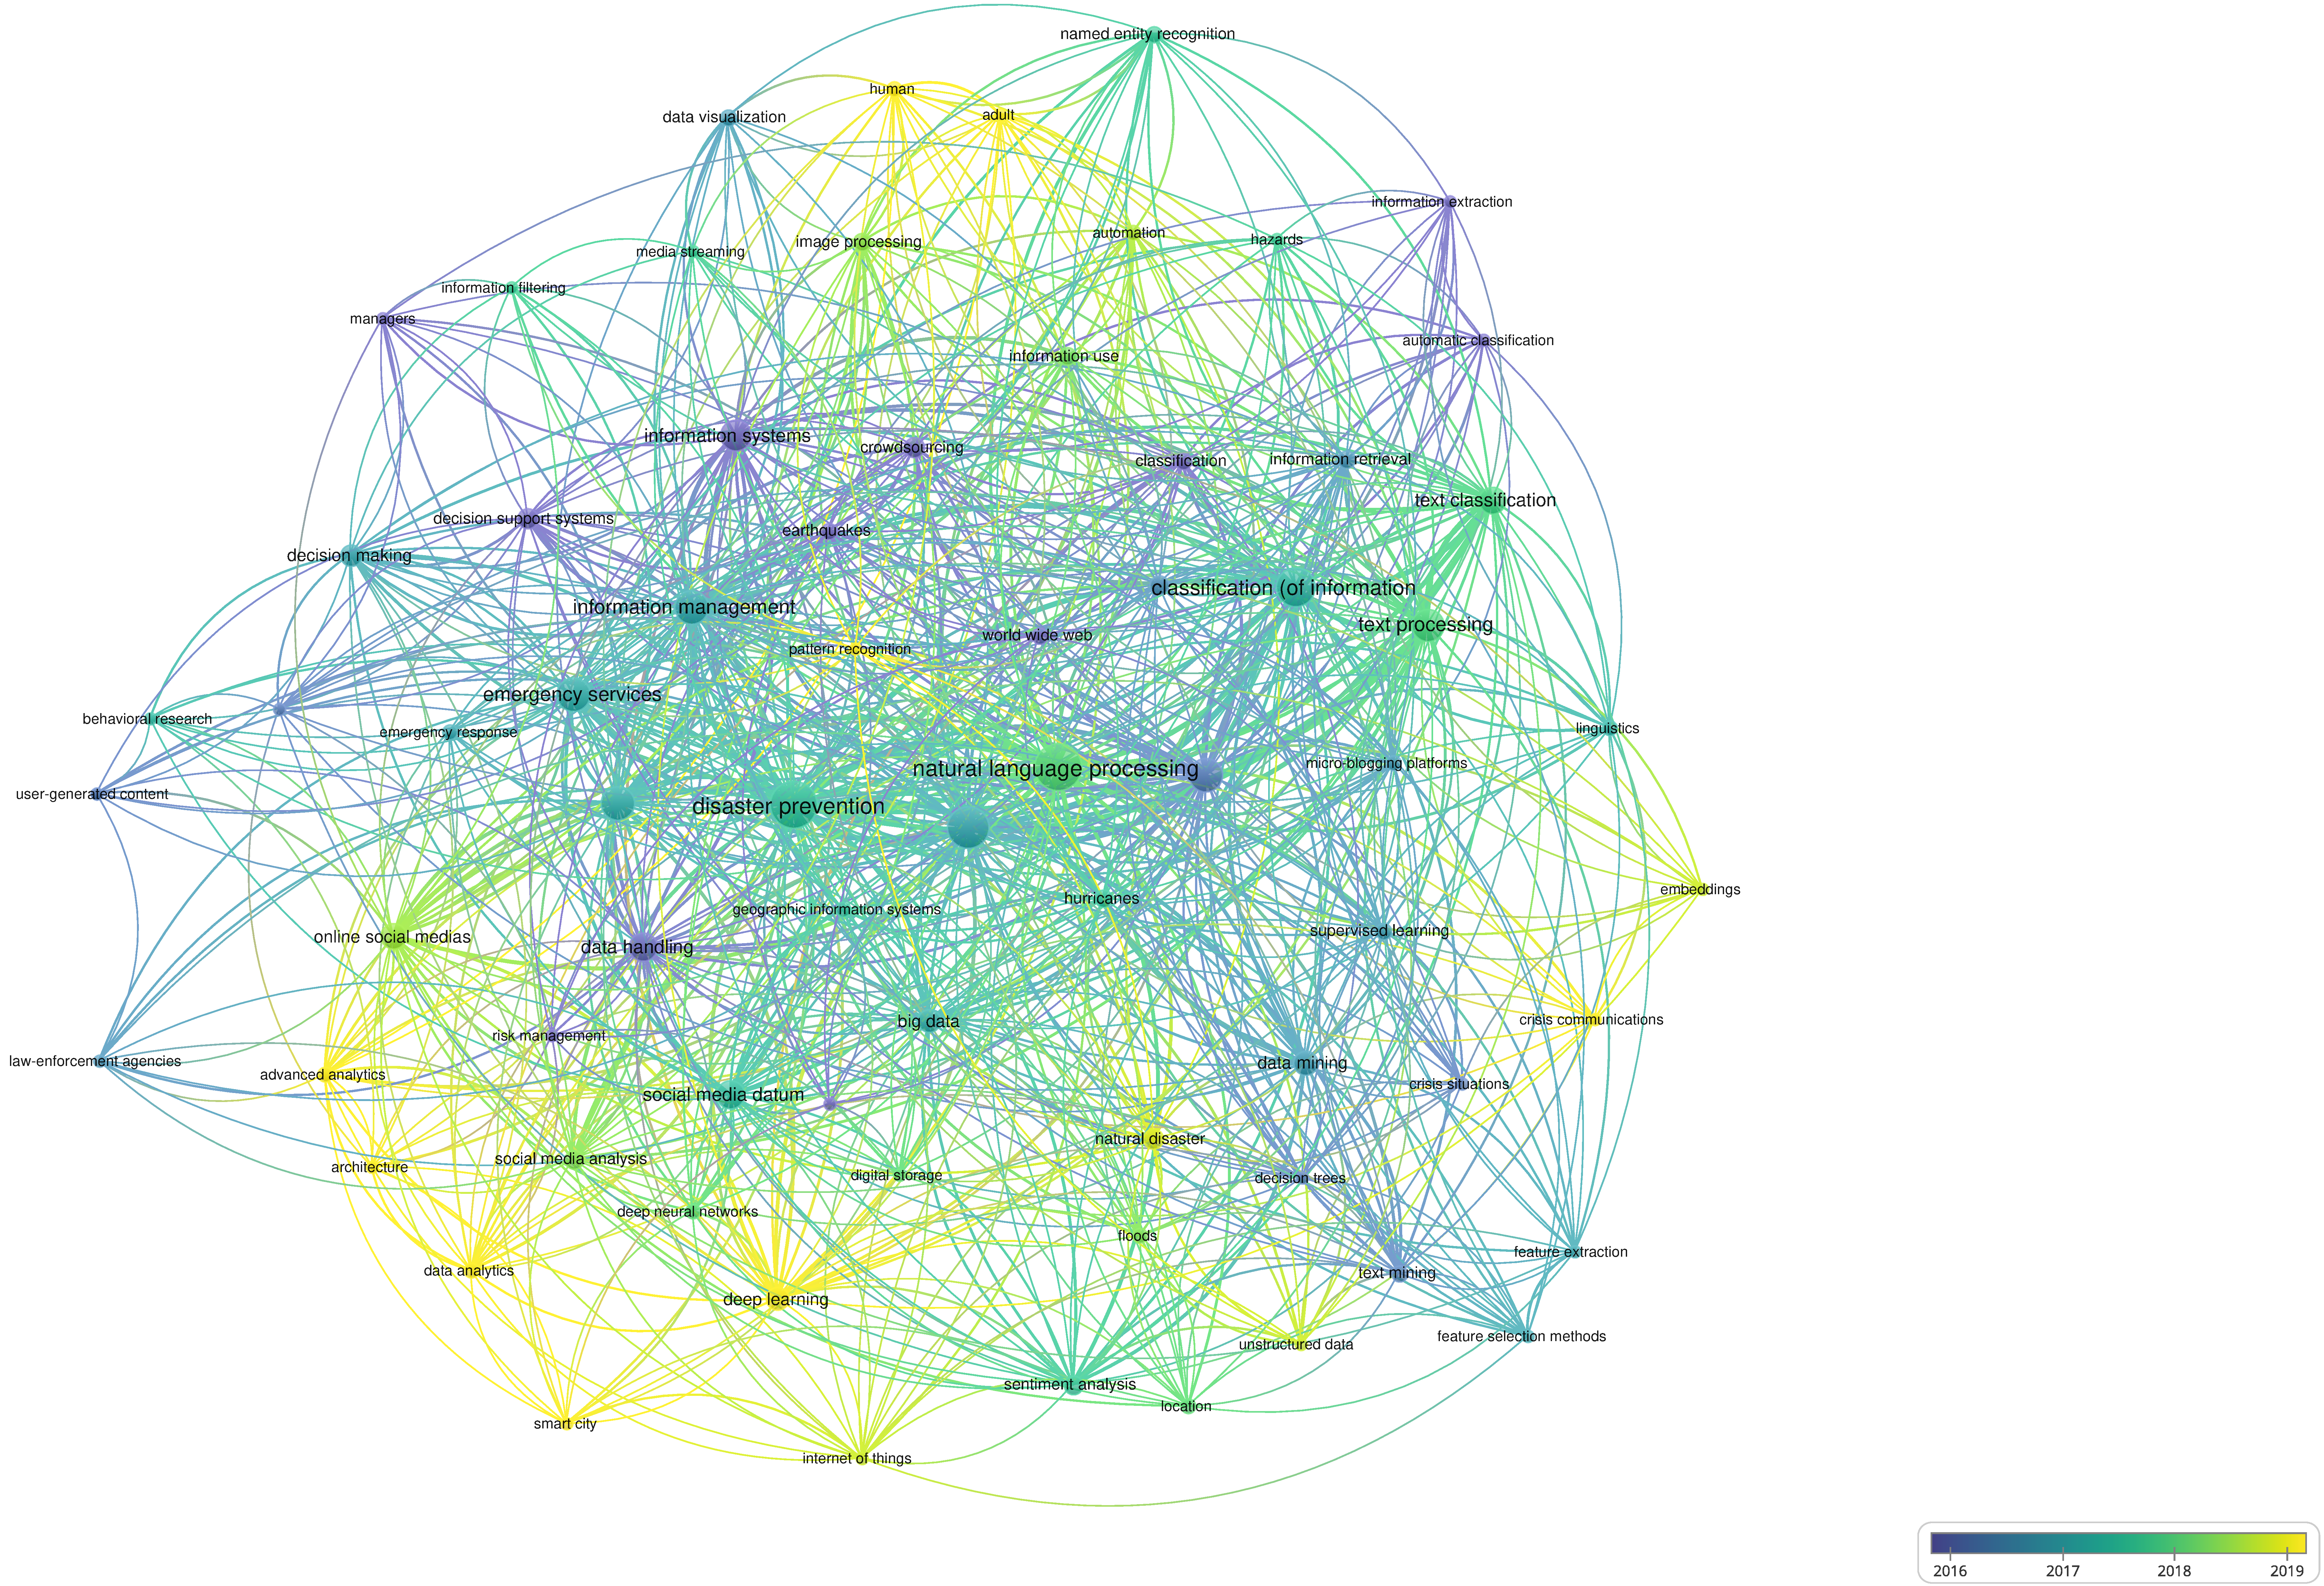
\includegraphics[width=\paperwidth,height=\paperheight,keepaspectratio]{figures/chap-2/crisis-informatic-overlay.pdf}
        \caption{Distribution of keywords with more than 3 occurrences among the articles from the query on crisis informatics. }
        \label{literature:crisis-informatic-overlay}
    \end{figure}
\end{landscape}

The bar diagram (Figure~\ref{literature:crisis-informatic-bar}) provides a better representation of the distribution of the occurrences of the different keywords.
From the most common ones, two areas of interest seem to emerge.
The automatic processing of the data, mostly textual according to the use of "natural language processing" and "text processing" is no more important than the use of this automation.
"Disaster prevention", "situation awareness", "information management" and "emergency services" highlight the importance of the applications of the results.

\begin{figure}[htb]
    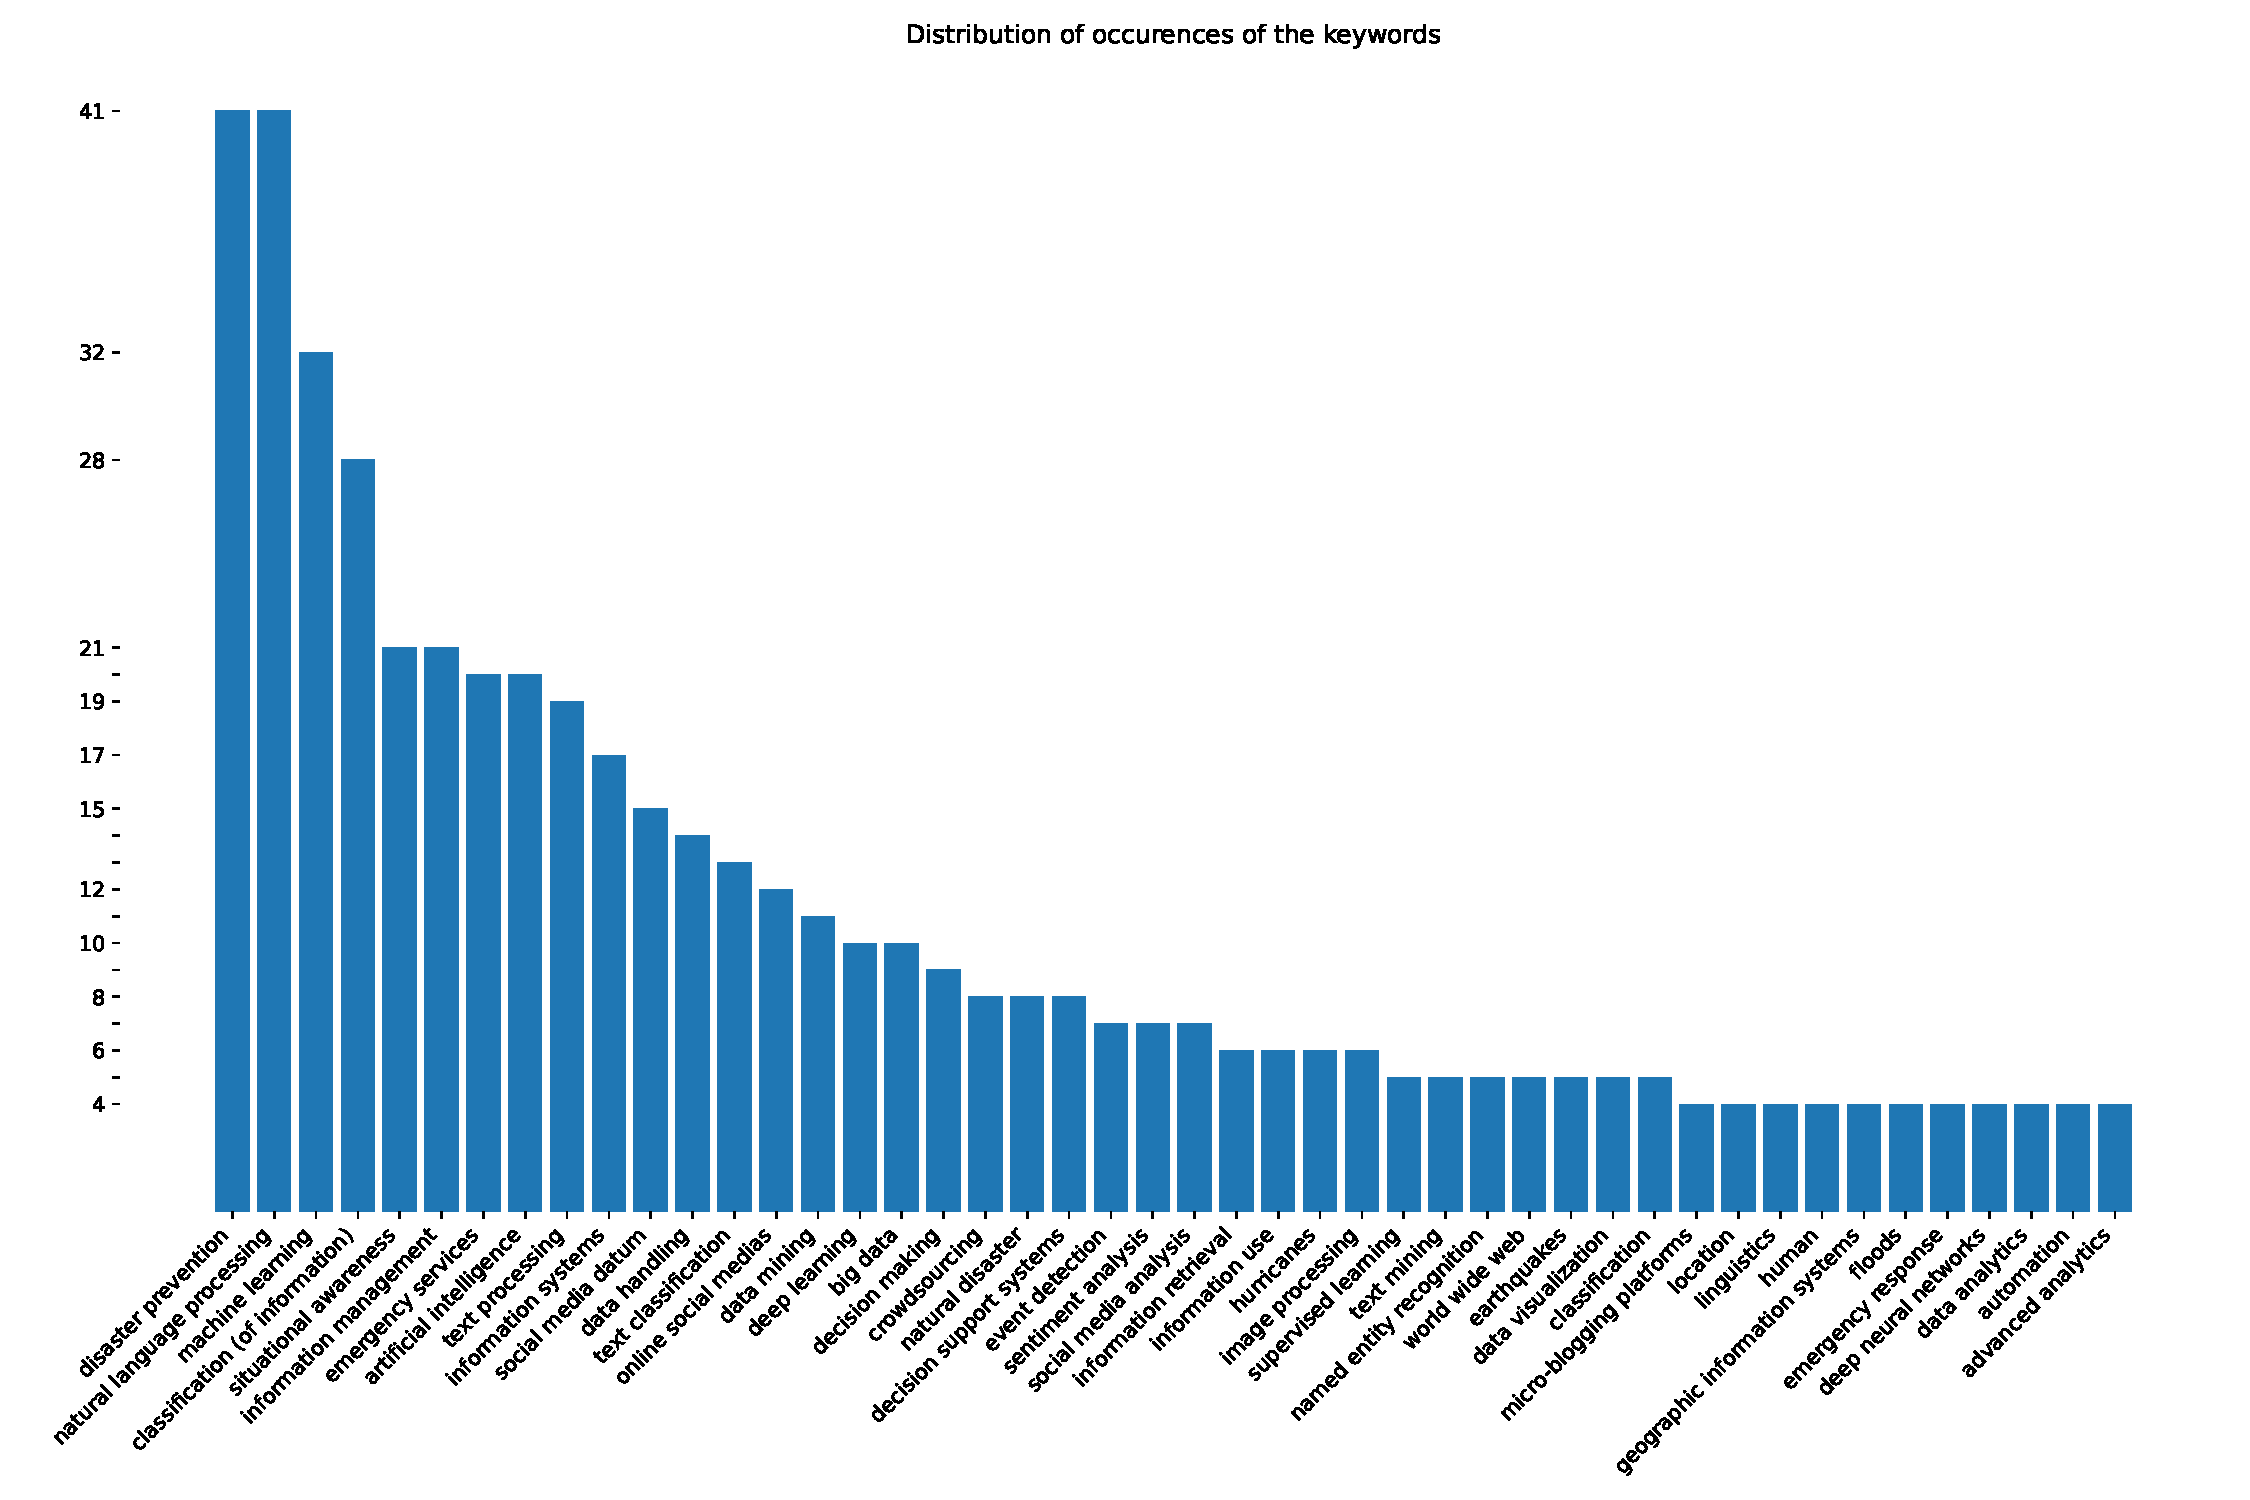
\includegraphics[width=\textwidth]{figures/chap-2/crisis-informatic-bar.pdf}
    \caption{Distribution of keywords with more than 3 occurrences among the articles from the query on crisis informatics. }
    \label{literature:crisis-informatic-bar}
\end{figure}

As mentioned in the first chapter, automatically processing the content of social media to extract information is a new and promising scientific venue.
Thus, many attempted to create systems to achieve this goal, proposing features to improve systems' usability.
Overview of the different attempts and their feature, to identify what have been done in this area.
Table~\ref{table:crisis-informatic-main-articles} presents the results of the previous query that mention a processing system that uses social media as a data source and that have been cited at least ten times are shown.
From these main systems, were extracted the main features presented by their authors.

Among the features identified, the trend towards automation observed earlier is still clear.
The first works present systems that use crowdsourcing to identify relevant information from messages posted on social media
(\cite{schulzCrisisInformationManagement2012a, backfriedOpenSourceIntelligence2012a, imranAIDRArtificialIntelligence2014b}).
The following works were interested in automating the previous tasks, presumably to reduce the dependence on human actors and to improve the processing of the important amount of data.
Problems related to the detection of occurence of events and their related information on social media, have been explored using different approaches (\cite{imranAIDRArtificialIntelligence2014b,middletonRealtimeCrisisMapping2014a,avvenutiEARSEarthquakeAlert2014a, gibsonCombiningBigSocial2014a}).
In parallel, experiments were conducted to identify the best ways to organize and disseminate the information obtained (\cite{middletonRealtimeCrisisMapping2014a,huangDisasterMapperCyberGISFramework2015a,avvenutiPullingInformationSocial2016a,grunder-fahrerTopicsTopicalPhases2018a}).
Building on its successes, the field has continued to develop by relying on other available data formats and in particular images (\cite{alamImage4ActOnlineSocial2017a,nguyenAutomaticImageFiltering2017a,agarwalCrisisDIASMultimodalDamage2020a}).
Beyond the data, new questions have emerged, following feedback from the emergency departments involved in the experiments.
The detection of sub-events and of the different concerns of the impacted population are added to the results of previous works (\cite{wuStreamExplorerMultiStageSystem2018a,raginiBigDataAnalytics2018a,grunder-fahrerTopicsTopicalPhases2018a}).
More recently, teams with a broader vision are interested in the integration of such systems within the connected city (\cite{shahDisasterResilientSmart2019a}).
The multiplication of sources and formats naturally leads to the need for unified processing methods for data and fusion of information obtained by the different channels (\cite{alamDescriptiveVisualSummaries2020a}).

\begin{table}[bp]
    \centering
    \renewcommand{\arraystretch}{1.5}
    \caption{Articles retrieved from the previous request which propose social media processing systems or methods with at least 10 citations.}
    \begin{tabular}{m{0.3\textwidth} m{0.2\textwidth} m{0.5\textwidth}}
        Reference                                        & Type of event studied & Features                                                 \\ [0.5ex]
        \toprule
        \cite{schulzCrisisInformationManagement2012a}    & None                  & Crowdsourcing                                            \\
        \cite{backfriedOpenSourceIntelligence2012a}      & None                  & Crowdsourcing, Automatic processing                      \\
        \cite{imranAIDRArtificialIntelligence2014b}      & None                  & Crowdsourcing, Information categories, Message filtering \\
        \cite{middletonRealtimeCrisisMapping2014a}       & None                  & Common Operational Picture, Location inference           \\
        \cite{avvenutiEARSEarthquakeAlert2014a}          & Earthquake            & Event detection                                          \\
        \cite{gibsonCombiningBigSocial2014a}             & None                  & Formal concept analysis, Rule-based method               \\
        \cite{glasgowOurGriefUnspeakable2014a}           & None                  & Death-related content detection                          \\
        \cite{huangDisasterMapperCyberGISFramework2015a} & None                  & Big Data, Common Operational Picture                     \\
        \cite{avvenutiPullingInformationSocial2016a}     & Earthquake, Flooding  & Event detection, Message filtering, Disaster management  \\
        \cite{alamImage4ActOnlineSocial2017a}            & None                  & Image processing, Infrastructure damage                  \\
        \cite{fersiniEarthquakeManagementDecision2017a}  & Earthquake            & Message filtering, Information management                \\
        \cite{nguyenAutomaticImageFiltering2017a}        & None                  & Image processing, De-duplication, Image filtering        \\
        \cite{raginiBigDataAnalytics2018a}               & Flooding              & Sentiment analysis                                       \\
        \cite{shahDisasterResilientSmart2019a}           & Earthquake, Tsunami   & Smart Cities, IoT integration                            \\
        \cite{grunder-fahrerTopicsTopicalPhases2018a}    & None                  & Topic modeling, Disaster management                      \\
        \cite{wuStreamExplorerMultiStageSystem2018a}     & None                  & Subevent detection, Clustering                           \\
        \cite{agarwalCrisisDIASMultimodalDamage2020a}    & None                  & Damage identification, Severity detection                \\
        \cite{alamDescriptiveVisualSummaries2020a}       & Hurricane             & Information fusion                                       \\
        \bottomrule
    \end{tabular}
    \label{table:crisis-informatic-main-articles}
\end{table}

%TODO Conclusion of the section

\section{Decision making in crisis situation: information needed}
This first part of the literature review tackles the first sub problematic: What information that can be obtained from social media is relevant to the decisiom makers in crisis response?
Its looks at answers at the question: \emph{what information is relevant to the decisiom makers in crisis response?}

Information are at the heart of the decision making process (references to the decision making processs + figure to summarize the whole process)
In order to make decisions, the decision maker will look for information on certain elements.
What are these information?

The first part of this literature review will look at different attempts to model the information needed in crisis response, from a decision maker point of view.
This part only consider the models that consider in their scope the stakes of crisis management identified in the first chapter: improve coordination and/or situational awareness.

\subsection{Information identified for crises: crisis situation models}
Crisis management is not a novel issue.
Thus, many tackled the problems in this area.
With the apparition of informatic as a way to delegate tasks, many thought about deligating a part of crisis management to the machine.
However, managing this information require at first to build representations of the crises for the computers.
Consequently, ontologies and information models emerged to represent the informational concepts manipulated during an emergency situation.
This subsection aims at retrieving from the literature the different key informational concepts, useful for decision makers during crisis response.

The request run on Scopus is as follow:
\begin{itemize}
    \item SUBJAREA(comp)
    \item AND (TITLE-ABS-KEY ({crisis management} or {crisis response} or {disaster management} or contingency or {disaster response}))
    \item AND (TITLE-ABS-KEY (ontology or metamodel))
    \item AND (EXCLUDE (DOCTYPE,"re") OR EXCLUDE (DOCTYPE,"cr"))
\end{itemize}

The request returns papers that:
\begin{itemize}
    \item Are in the computer science domain, as this domain contains both the AI and Information Systems domains.
    \item Are centered around crises|disasters management|response or contingency plans.
    \item That present systems that process data
    \item Papers that present conference tracks and reviews are excluded.
\end{itemize}

The request returns 205 documents, published between 1998 and 2021.
Figure~\ref{literature:situation-models-hist} shows the evolution of the volume of publication between 1998 and 2020.
The field has emerged around 2000 and built momentum during ten years to reach a plateau a mean of around fifteen articles per years to these days.
The domain developped in order to organize the data, information and knowledge present during crisis events.
To achieve this goal, representions of the different concepts involved during such events were needed.
Two paths to represent these concepts have been taken: ontologies and metamodels.
Ontologies and metamodels are very close concepts.
Both methods aim at creating a controlled vocabulary to define the entities and their relations in a given domain.
The difference between the two methos happens at the grammar used for the vocabulary.
Metamodels usually use a formal and common grammar (a modelisation language such as UML) to ease the distribution and development of these representation.
Metamodels, as the backbone of model driven engineering, tend to be developped with interoperability between different systems in mind.
Thus the use of common tools to represent concepts between the engineers.
Ontologies, on the other hand, use their own grammar for the entities that its define.
As mentioned in the first chapter, crises are a were wide concept and the creation of ontologies or metamodels of crisis situations is a very challenging task.
Thus, many ontologies and metamodels have been created to represent different aspects of crisis management.

\begin{figure}[bp]
    \centering
    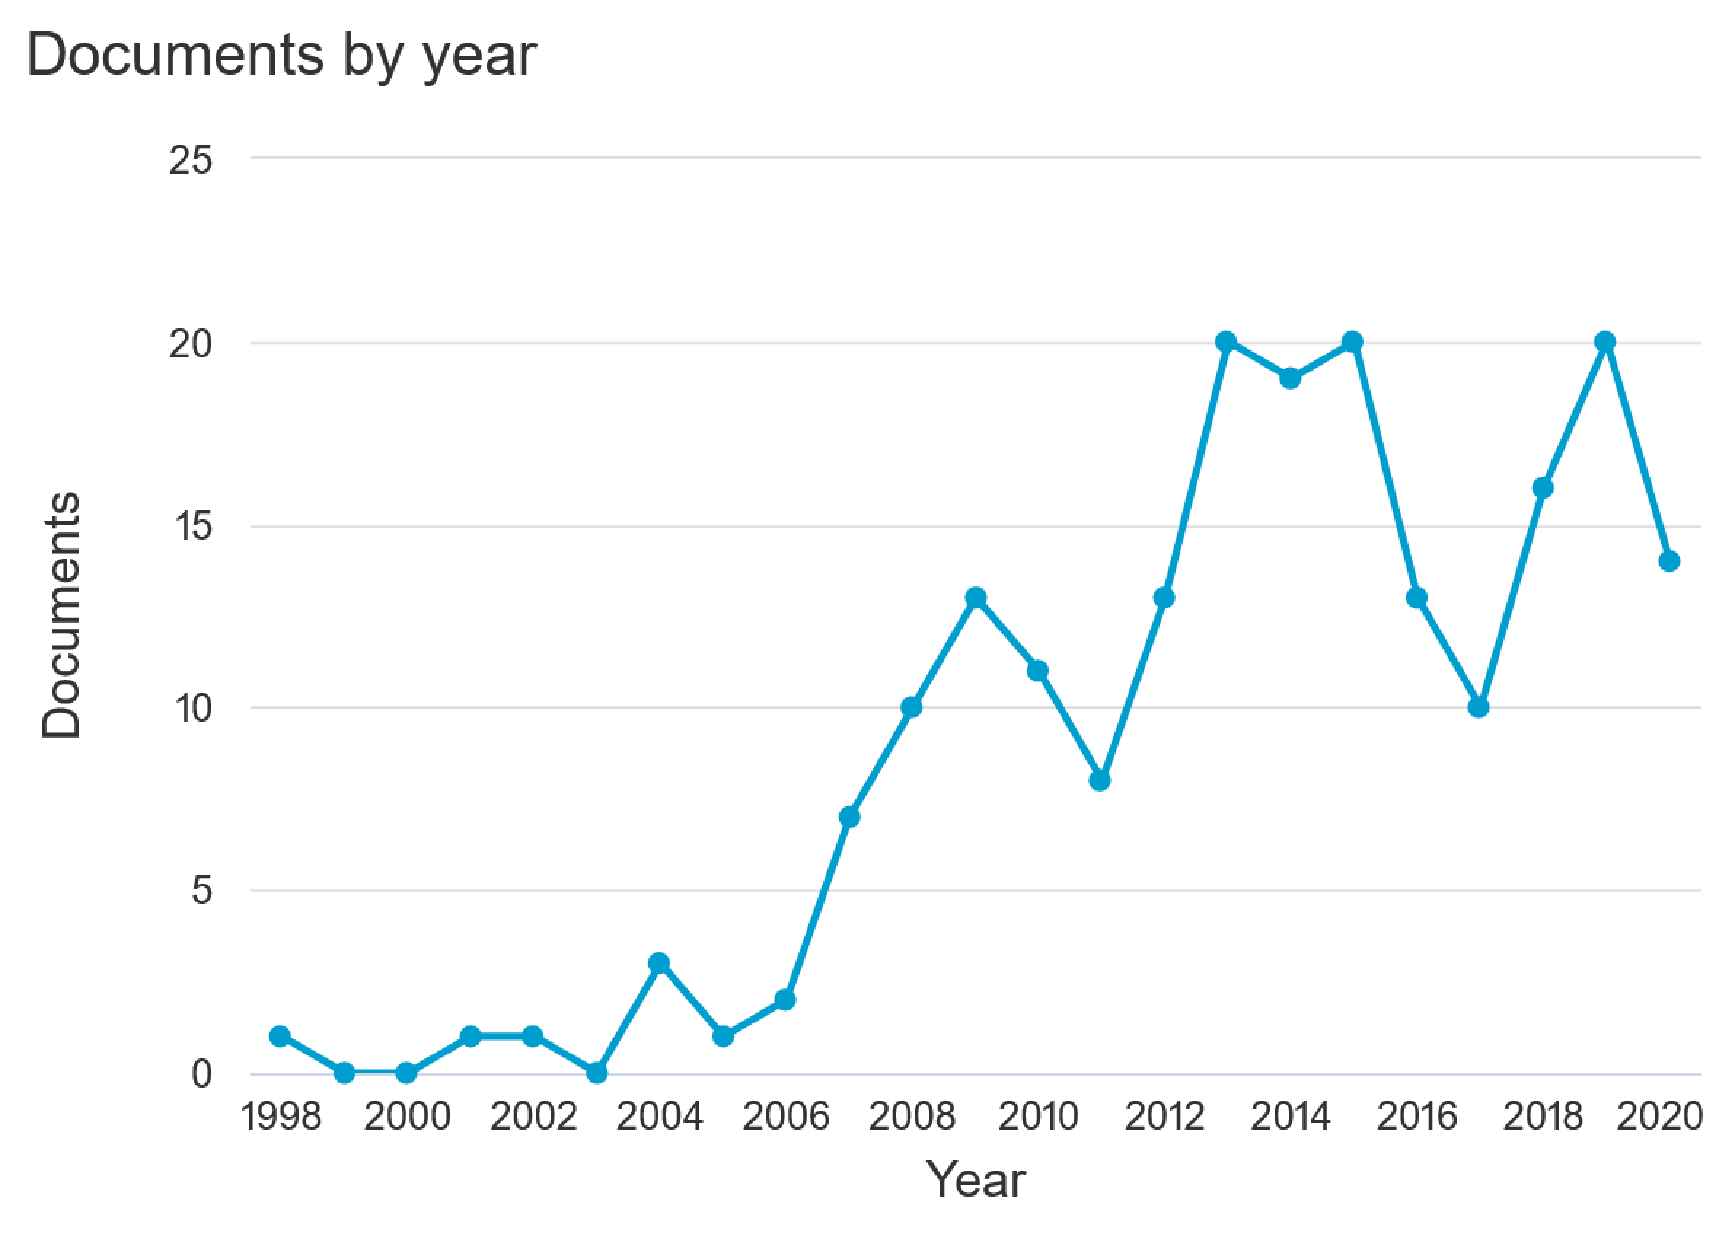
\includegraphics[width=\textwidth]{figures/chap-2/situation-models-hist.pdf}
    \caption{Timelime of the volume of contributions per years for the crisis-situation models domain. The year 2021 is excluded because the year is not complete at the time of writing.}
    \label{literature:situation-models-hist}
\end{figure}

Following the same methodology as in the previous section, Figure~\ref{literature:/situation-models-overlay} provides a visual of the evolution over time of the different keywords used in the fetched articles.
The overlay indicates three clusters: a major one and two smaller ones.
One is related to genes and the other one is related to supply chains and infrastructures.
The one related to genes is a cluster of outliers, composed of 7 articles from the medical field.
The second cluster is also composed of few articles centered around ontologies for the petroleum sector.
The main cluster however, is more centered on the topic of this literature review.
As in the previous section, the evolution (represented by the color variation) of the keywords hint at the direction of the domain over time.

\begin{figure}[bp]
    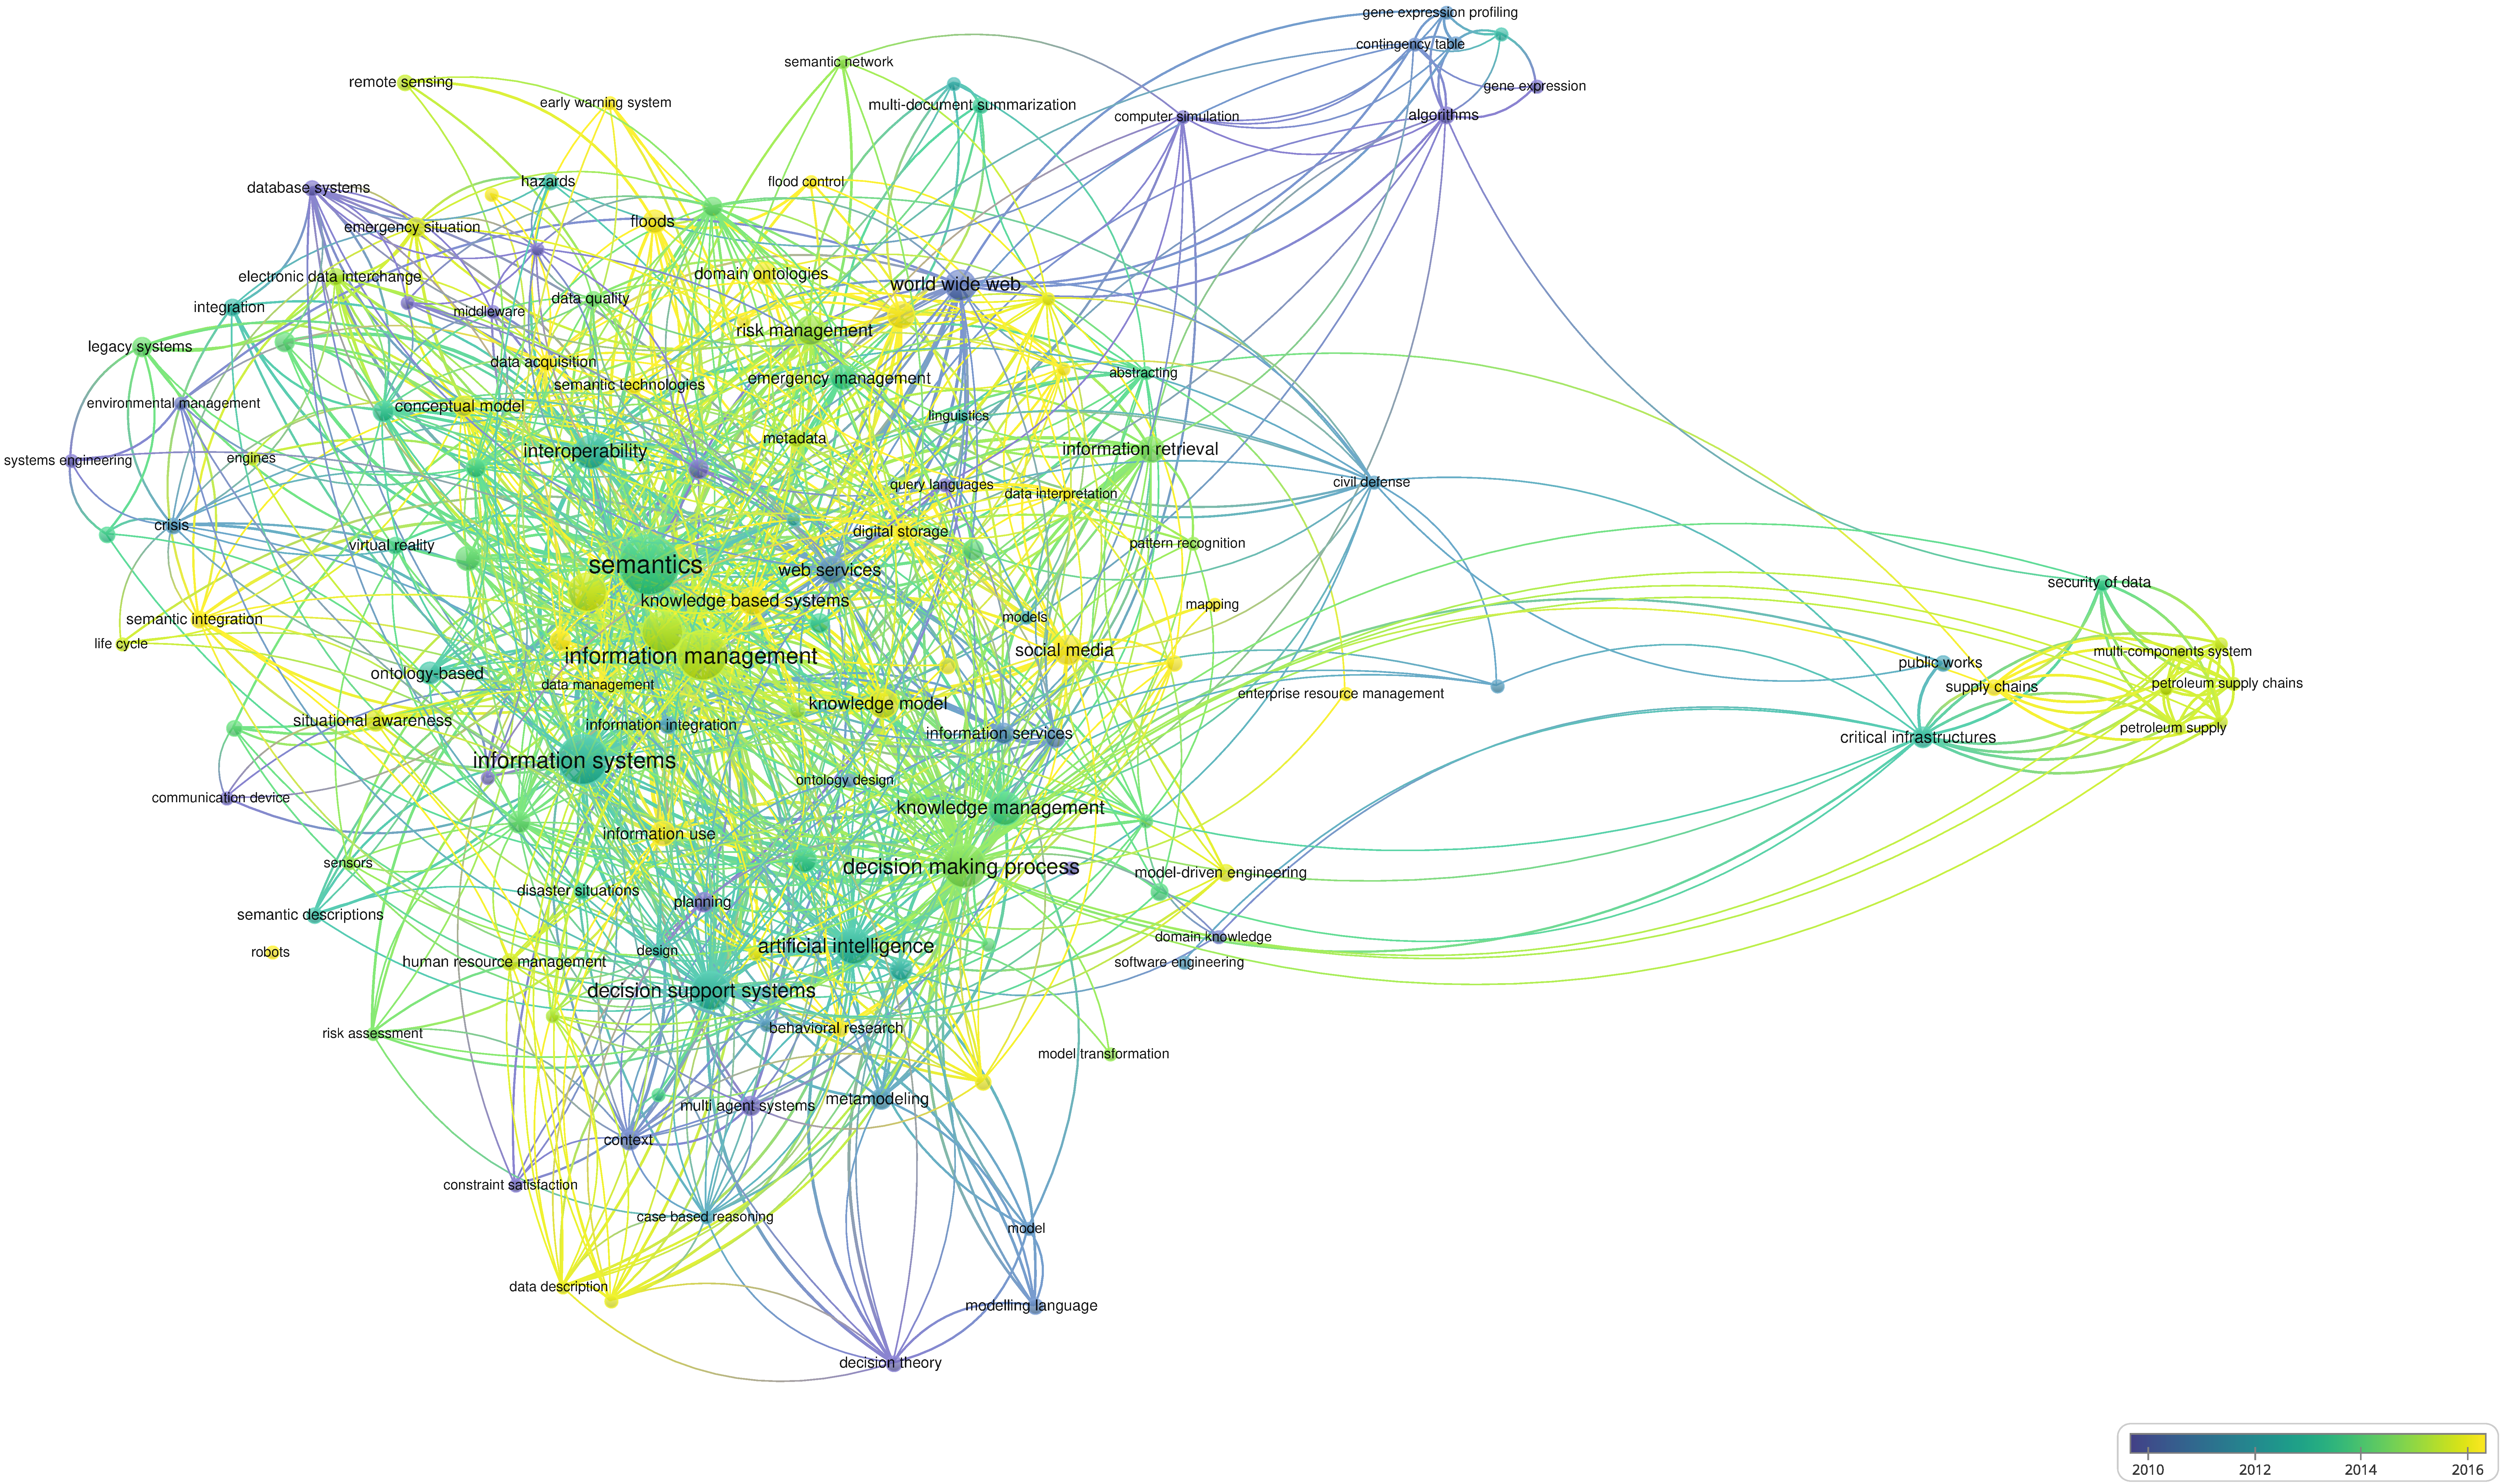
\includegraphics[width=\paperwidth,height=\paperheight,keepaspectratio, angle=90]{figures/chap-2/situation-models-overlay.pdf}
    \caption{Distribution of keywords with more than 3 occurrences among the articles from the query on crisis-situation models.}
    \label{literature:/situation-models-overlay}
\end{figure}

Unlike the query, the overlay spans from 2010 to 2016. This is because the overlay does not include all keywords, but only those that appear in at least 3 different articles.
By cross-checking this information with the previous histogram, one understands the reason for this short period.
For many years the number of publications was relatively low, and apparently without any real consensus among the keywords.
If this is understandable at the beginning of a field, this explanation does not explain the stop of the overlay from 2016.
However, using again the histogram, one notices that the domain loses popularity from 2015 onwards to return to its previous level around 2018.
It is possible to hypothesize that it is this loss of interest that has led to the result observed on the overlay.

Despite this short span covered, it is possible to identify trends in keywords use somehow similar to the ones in crisis informatic.
The older keywords used, such as "SOA", "simulation", "multi agent systems" and "systems engineering" show an interest centered around the core of what were used ontologies and metamodels for: model driven engineering and information management.
Then, the field knew a pic of interest, as the previous histogram show.
This period reflects on Figure~\ref{literature:/situation-models-bar}, where one can observe that most of the most importants keywords are located between 2012 and 2014.
As explained previously, the years between 2021 and 2014 were indeed the most prolific.
These years were mostly focused on the idea of crisis management systems, powered by artifical intelligence for decision support.
Artificial intelligence would automatically create the information representations needed by systems.
As these representations would have been written in a common fashion, these systems would have been able to quickly adapt to new representations, providing greater interoperability.
After this period, the interest in the field decrease a few, before coming back with new approaches.
Knowledge based systems and knowledge management started to appear, as well as a reborn of metamodel and ontologies creation, powered by improvements in machine learning.

\begin{figure}[bp]
    \centering
    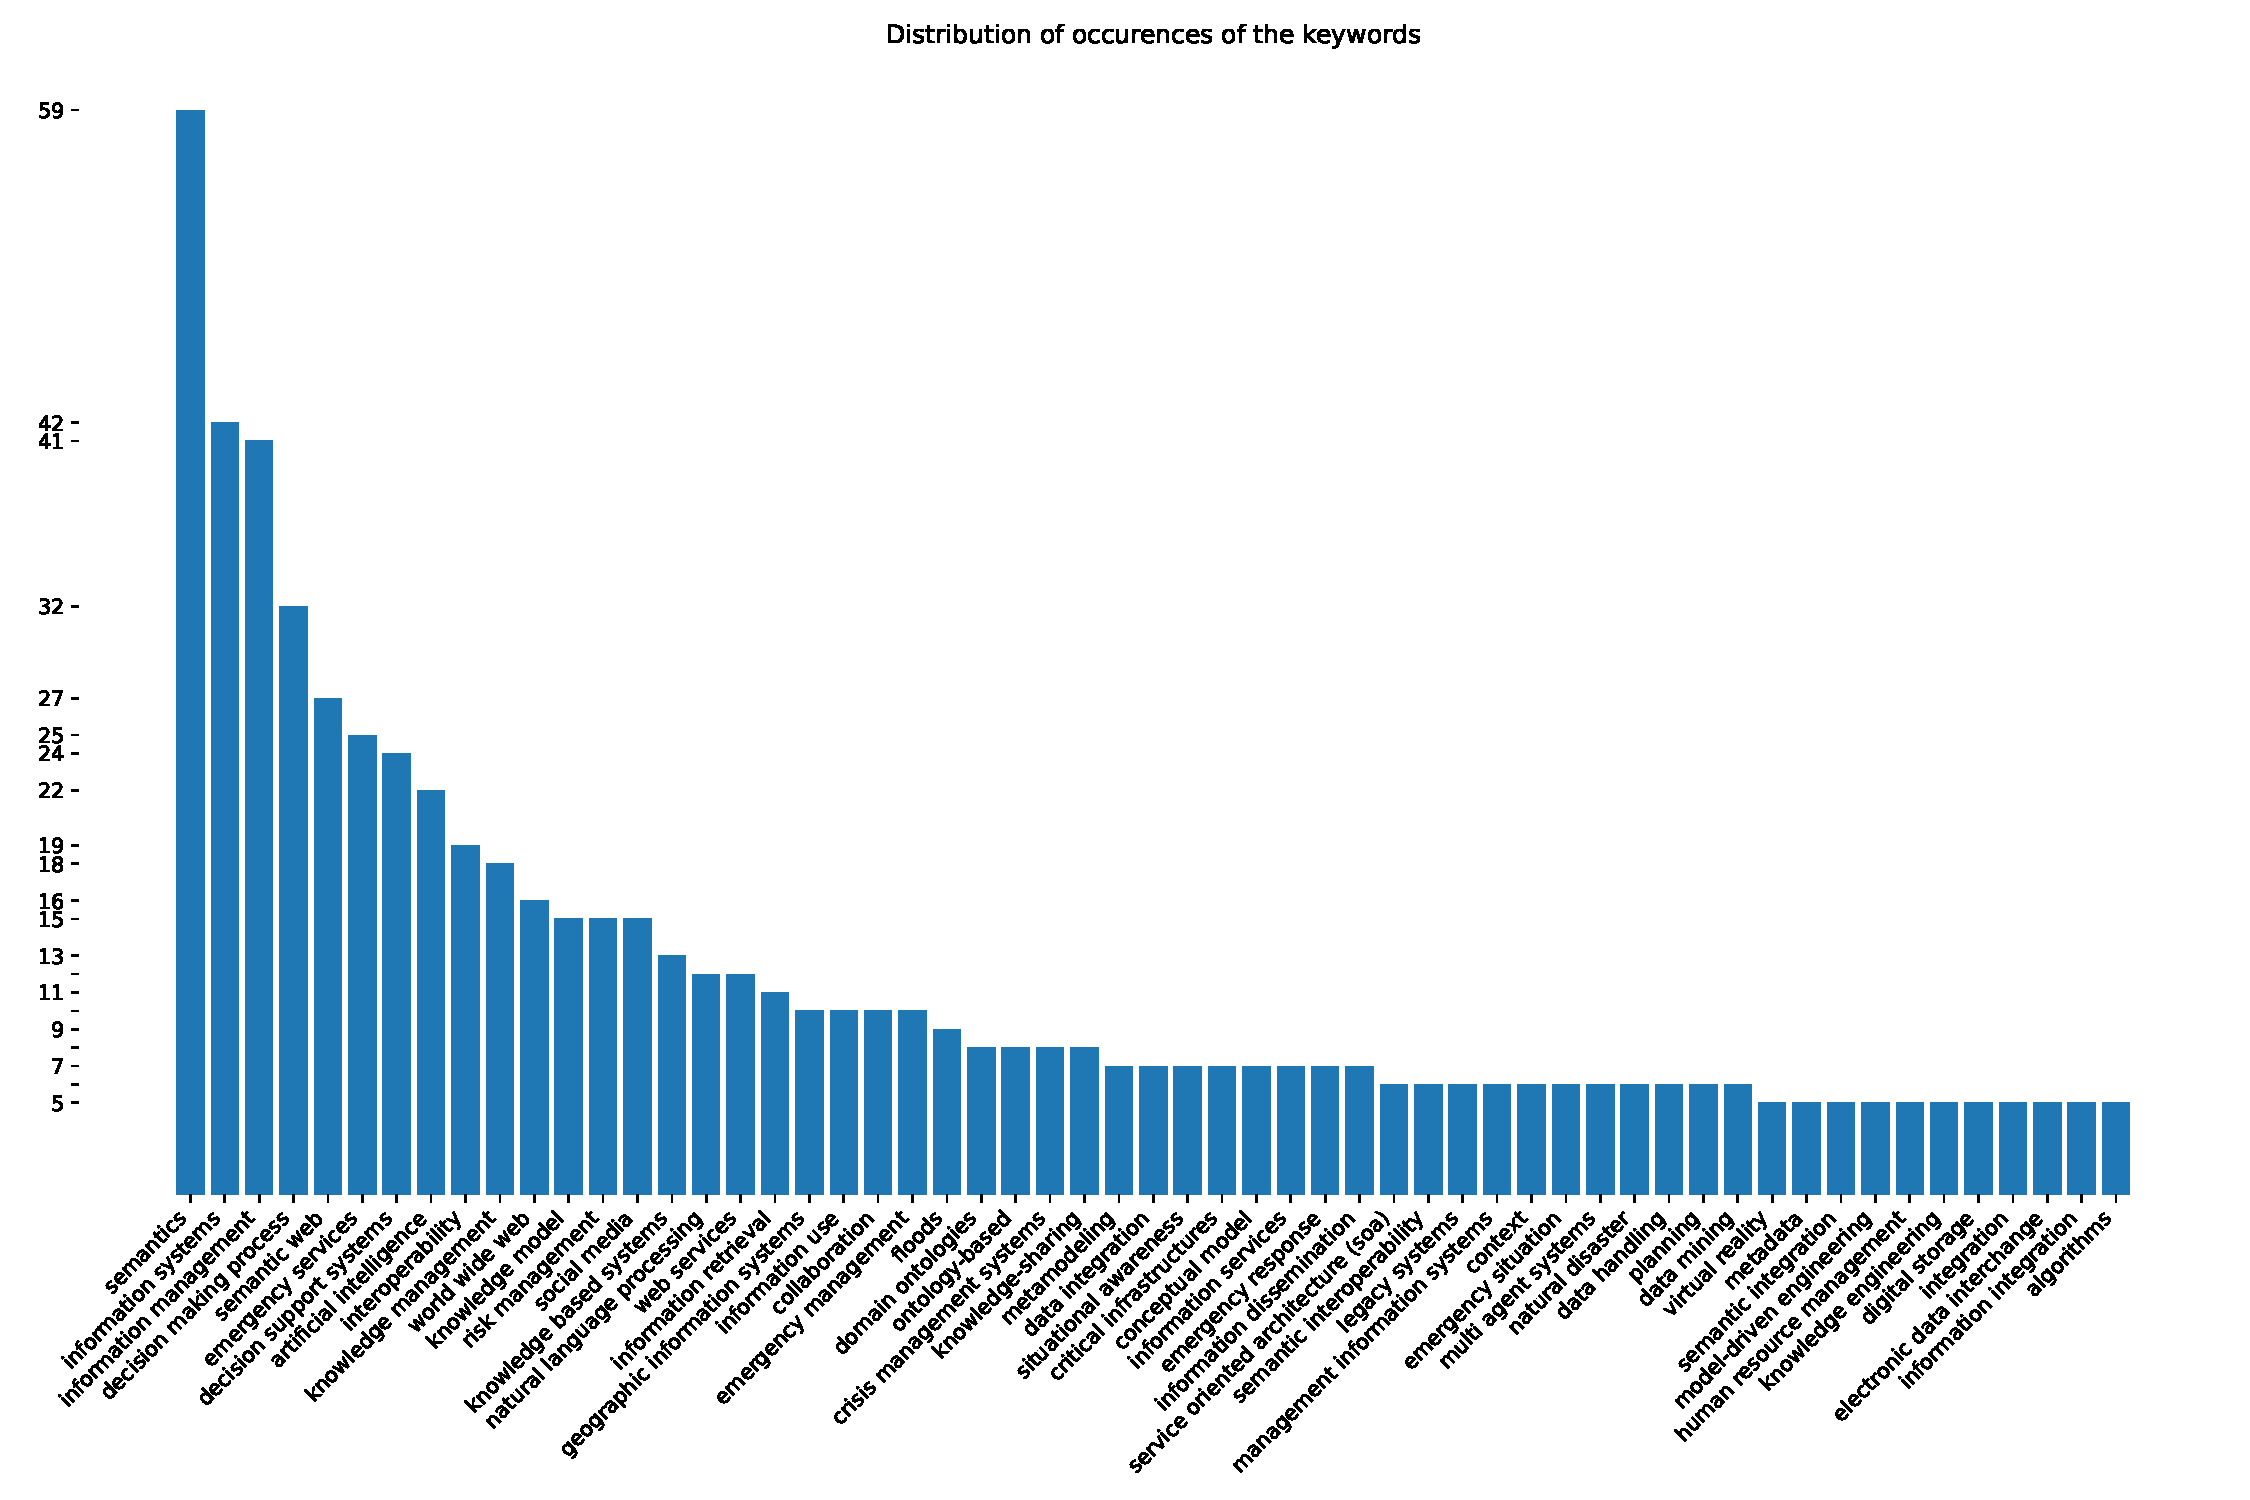
\includegraphics[width=\textwidth]{figures/chap-2/situation-models-bar.pdf}
    \caption{Distribution of keywords with more than 4 occurrences among the articles from the query on crisis-situation models.}
    \label{literature:/situation-models-bar}
\end{figure}

In association with the previous qualitative review of the field, Table~\ref{table:situation-models-main-articles} presents the decision makers needs identified in the articles from the previous request with at least 25 citations.
Duplicates and unrelated articles (e.g. gene ontologies) are also excluded.
This review of the main articles highlight the diversity of approaches covered by ontologies and metamodels.
Some of these ontologies are event specific (\cite{xuModelingRepresentationEarthquake2014a,qiuIntegratedFloodManagement2017a,jungOntologydrivenSlopeModeling2015a}).
While these models are effective at dealing with the event they are designed for, most of their concept representations do not fit with other kind of events.

Collaboration between the actors is, as presented in the introductory chapter, a matter of interest for crisis management organizations.
Thus (\cite{benabenMetamodelItsOntology2008b}) and (\cite{othmanDevelopmentValidationDisaster2014b}) propose metamodels to represent the collaboration between several actors, independantly of the type of crisis.

Others have also focused on emergency organization and proposed ways to improve their functioning.
\cite{chouOntologyDevelopingWeb2011a} proposed a way to automatically create websites to dissemination information related to an ongoing event.
As reports are an important concerns and participate to information overload, \cite{liOntologyenrichedMultiDocumentSummarization2010a} created an ontology to assist in report summarization.
Disaster management software are inherently complex. Thus, \cite{babitskiSoKNOSUsingSemantic2011a} proposed an ontology to assist in their development and another to assess their functionalities.
As disaster management systems grow, they become intricated and complex. \cite{madniSystemsIntegrationKey2014a} proposed an ontology to facilitate their integration into a functioning system of systems.

All the systems mentioned above require data.
Fortunately, sensors are excellent ways to keep emergency responders informed of certain caracteristics of their environment.
\cite{posladSemanticIoTEarly2015a} and \cite{babitskiOntologybasedIntegrationSensor2009a} proposed ontologies to better integrate sensors data into crisis cells.
Finally, another type of sensor considered are humans, acting as social sensors whose data can be automatically gathered from social media plateforms.
\cite{purohitIdentifyingSeekersSuppliers2014a} proposed an ontology to identify victims requests and volunteers capabilities from tweets.
As being able to geolocate the individual behind a post allows better actionability for emergency services, \cite{ghahremanlouGeotaggingTwitterMessages2014a} built an ontology to help solve this issue.

\begin{table}[bp]
    \centering
    \renewcommand{\arraystretch}{1.5}
    \begin{tabular}{m{0.25\textwidth} m{0.75\textwidth}}
        Reference                                                & Decision makers needs identified       \\ [0.5ex]
        \toprule
        \cite{benabenMetamodelItsOntology2008b}                  & Collaboration                          \\
        \cite{babitskiOntologybasedIntegrationSensor2009a}       & Sensor integration                     \\
        \cite{liOntologyenrichedMultiDocumentSummarization2010a} & Reports summarization                  \\
        \cite{babitskiSoKNOSUsingSemantic2011a}                  & Disaster management software usability \\
        \cite{chouOntologyDevelopingWeb2011a}                    & Automatic web sites creation           \\
        \cite{ghahremanlouGeotaggingTwitterMessages2014a}        & Location retrieval                     \\
        \cite{madniSystemsIntegrationKey2014a}                   & System integration                     \\
        \cite{othmanDevelopmentValidationDisaster2014b}          & Collaboration                          \\
        \cite{purohitIdentifyingSeekersSuppliers2014a}           & Identify victims and volunteers        \\
        \cite{xuModelingRepresentationEarthquake2014a}           & Earthquake management                  \\
        \cite{jungOntologydrivenSlopeModeling2015a}              & Landslide prevention                   \\
        \cite{posladSemanticIoTEarly2015a}                       & Sensor intregration                    \\
        \cite{qiuIntegratedFloodManagement2017a}                 & Flood management                       \\
        \bottomrule
    \end{tabular}
    \caption{Articles retrieved from the previous request which propose social media processing systems or methods with at least 25 citations.}
    \label{table:situation-models-main-articles}
\end{table}

This part identified the different approaches to model information in crisis response from a decision maker point of view.
Yet, most of these approaches are top-down, and few conducted interviews to directly identify decision makers needs'.
The next section looks at articles in the literature that used a bottom-up approach to identify the aforementioned needs.

\subsection{Business needs of emergency services}
Interviews and surveys have been conducted to identify what are the information needed by decision makers.
The goal of this section is similar to the one of the previous section, but considering a different approach.

Thus the aim is to remove the noise (needs that are too specific to certain domains) and the stop-needs (needs that are just way to vague and/or obvious).
Instance of vague ones: information, situational awareness etc.

Request:
\begin{itemize}
    \item SUBJAREA(comp)
    \item AND (TITLE-ABS-KEY ({crisis management} or contingency or {disaster response}))
    \item AND (TITLE-ABS-KEY (ontology or metamodel))
    \item AND (EXCLUDE(DOCTYPE,"re") OR EXCLUDE(DOCTYPE,"cr"))
\end{itemize}

Figure~\ref{literature:business-needs-hist}

\begin{figure}[bp]
    \centering
    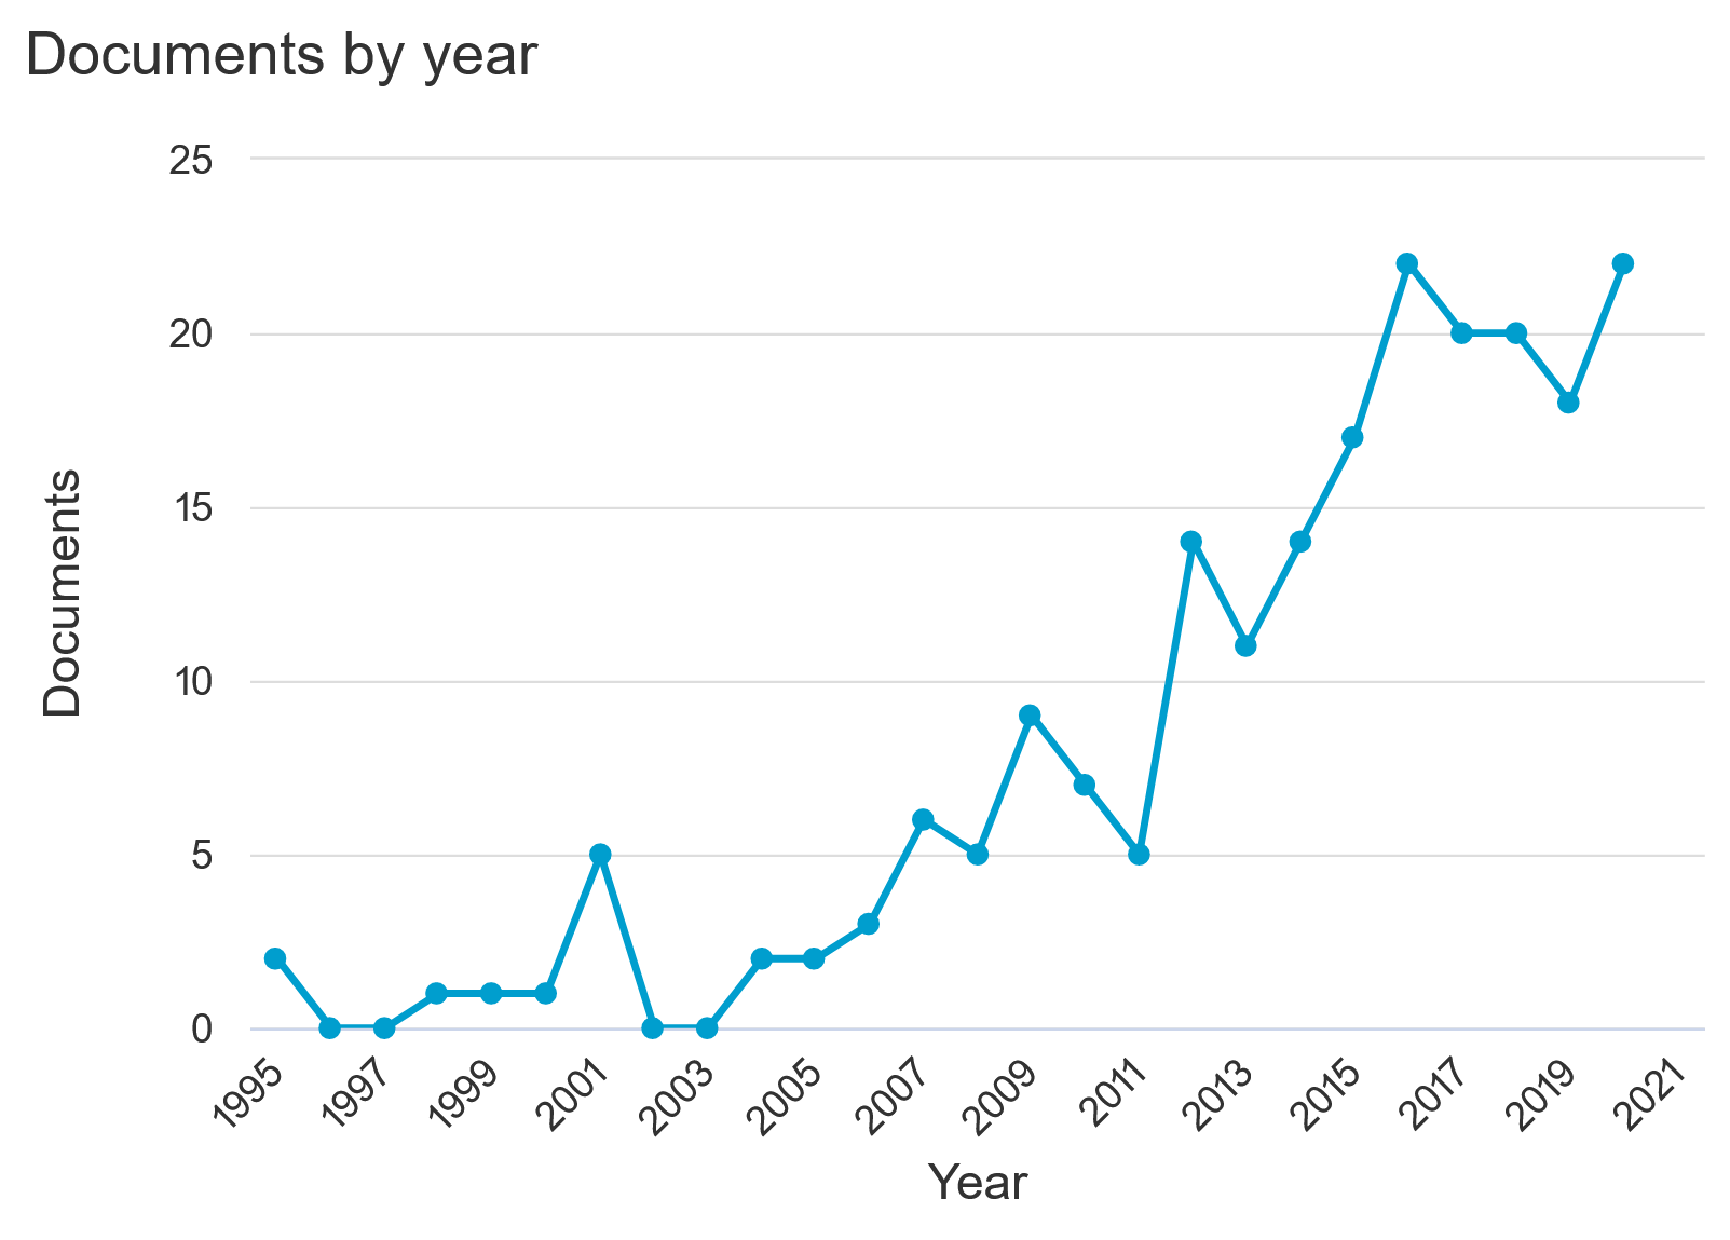
\includegraphics[width=\textwidth]{figures/chap-2/business-needs-hist.pdf}
    \caption{Timelime of the volume of contributions per years for the crisis informatic domain. The year 2021 is excluded because the year is not complete at the time of writing.}
    \label{literature:business-needs-hist}
\end{figure}

Figure~\ref{literature:business-needs-bar}

\begin{figure}[bp]
    \centering
    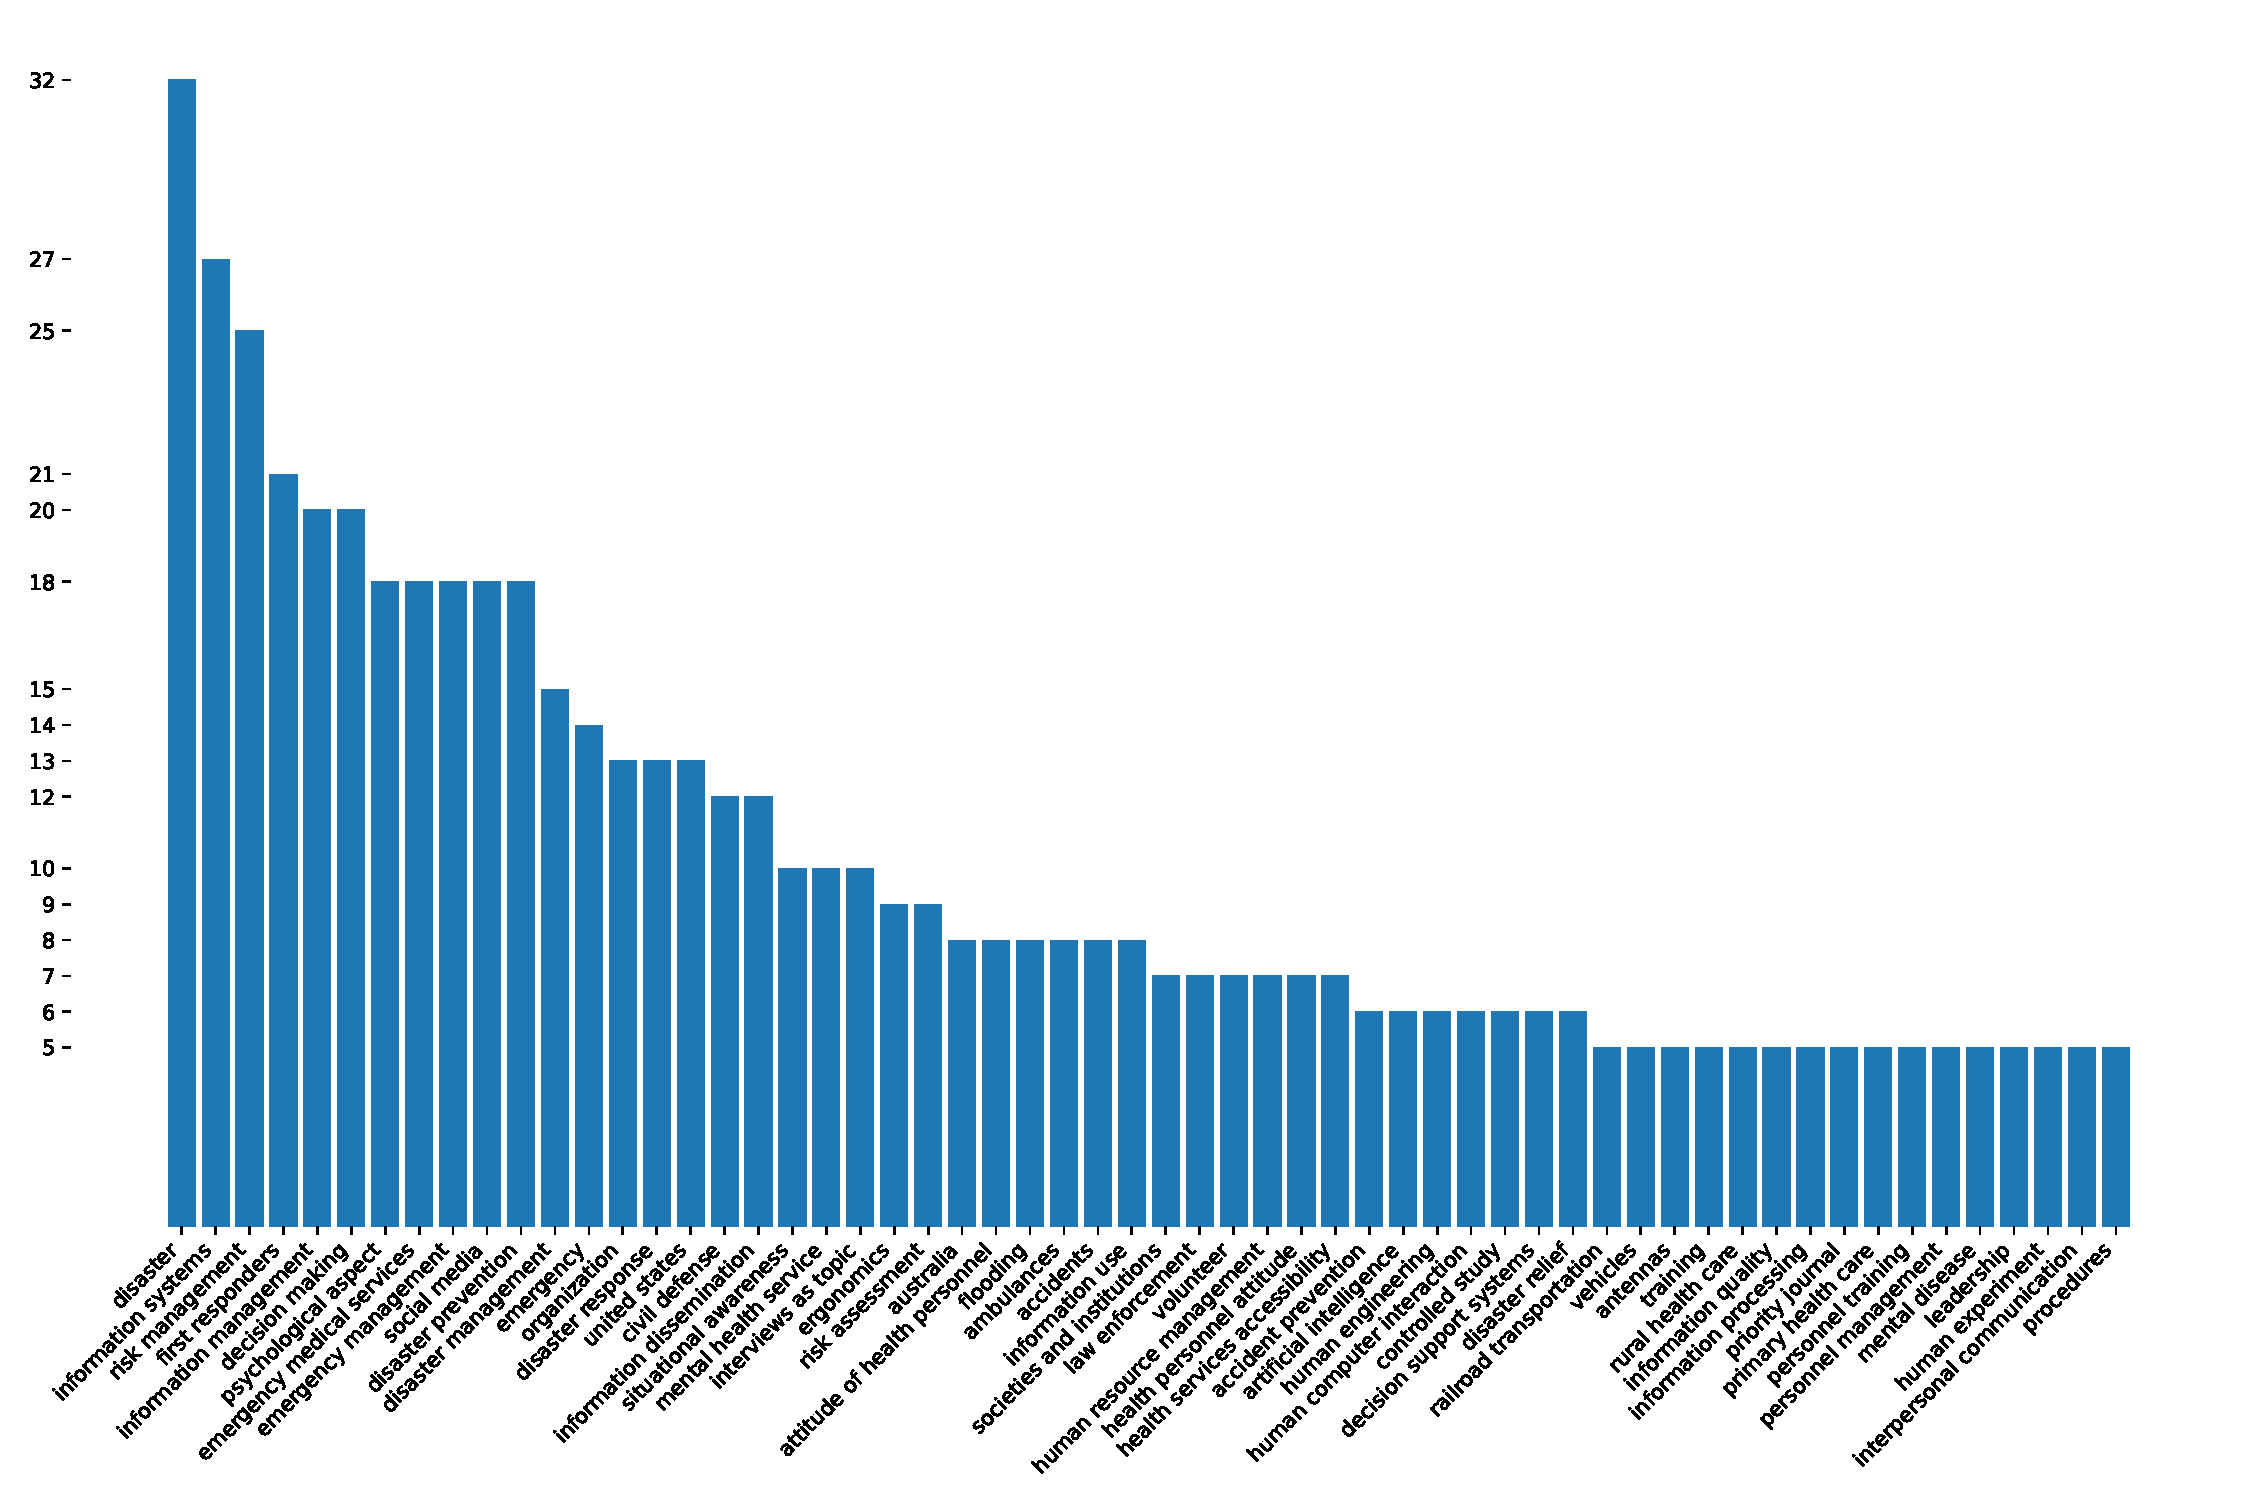
\includegraphics[width=\textwidth]{figures/chap-2/business-needs-bar.pdf}
    \caption{Distribution of keywords with more than 3 occurrences among the articles from the query on crisis informatics. }
    \label{literature:business-needs-bar}
\end{figure}

Figure~\ref{literature:business-needs-overlay}

\begin{figure}[bp]
    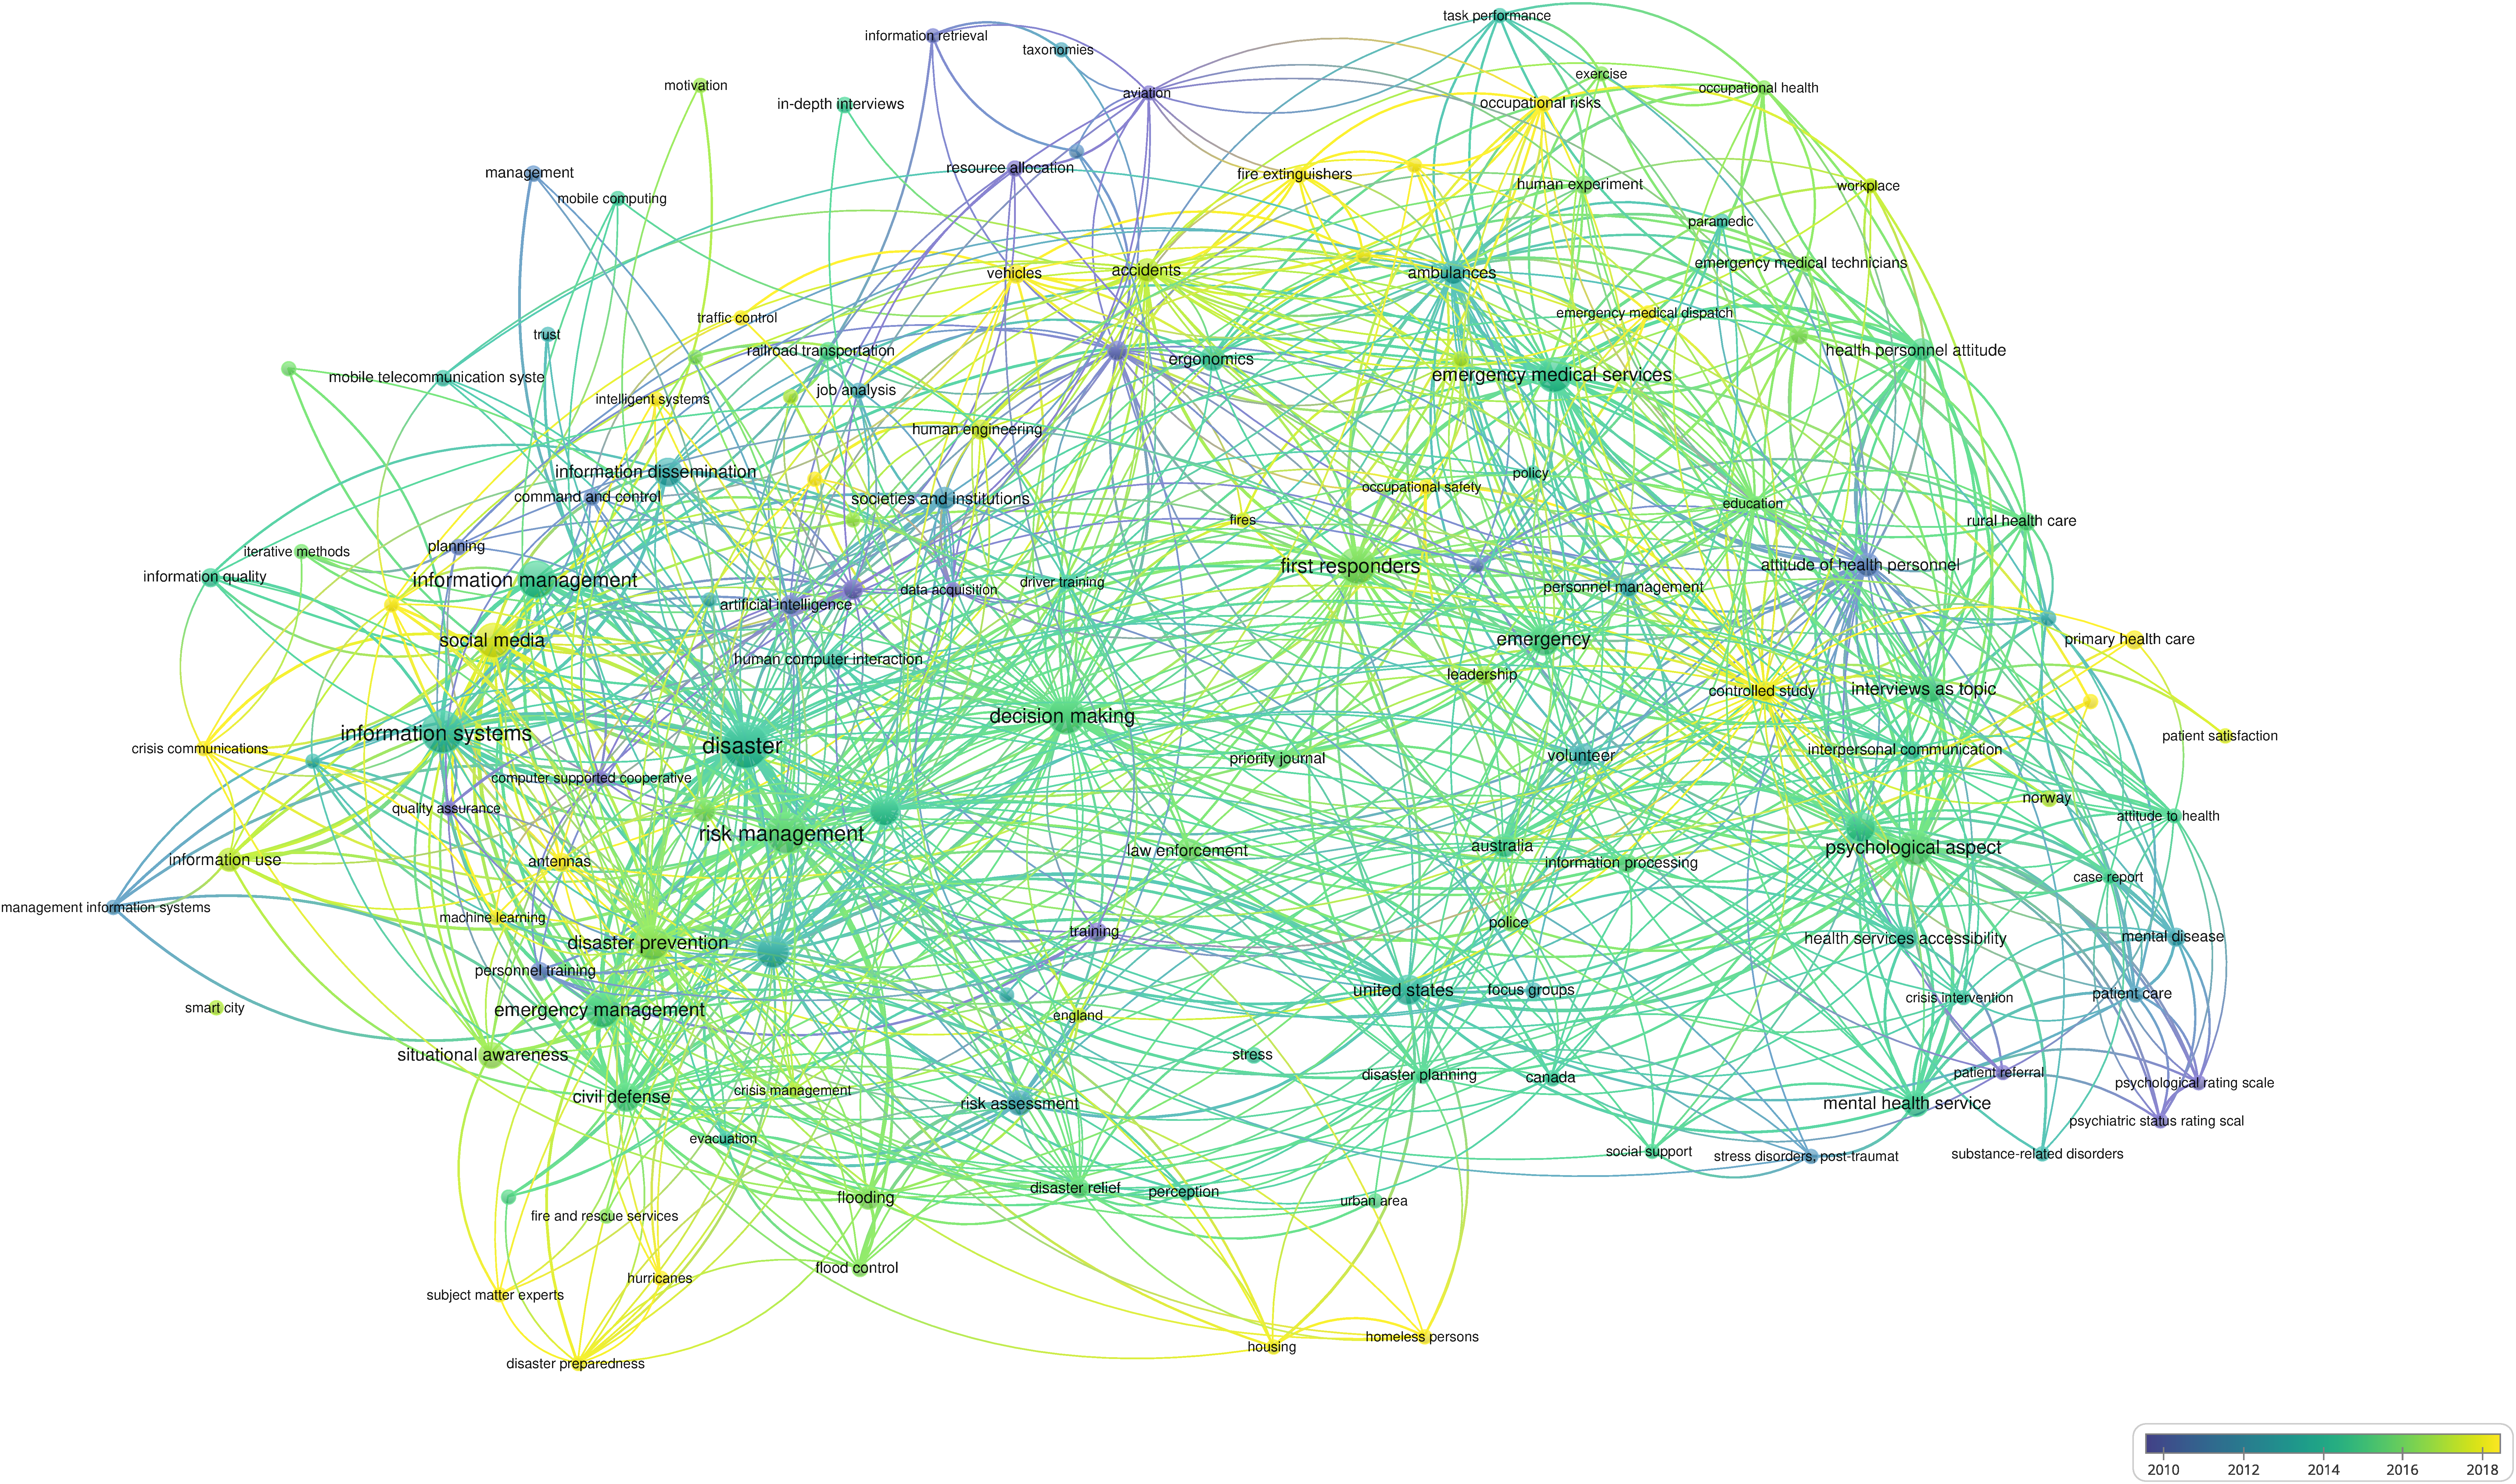
\includegraphics[width=\paperwidth,height=\paperheight,keepaspectratio, angle=90]{figures/chap-2/business-needs-overlay.pdf}
    \caption{Distribution of keywords with more than 3 occurrences among the articles from the query on crisis informatics. }
    \label{literature:business-needs-overlay}
\end{figure}

% Les articles partials ont été prit pour au moins 25 citations, comme pour les articles de les modeles de situations de crise.

""Decision makers information needs identified through interviews""

% Table~\ref{table:business-needs-main-articles}

% \begin{table}[bp]
%     \centering
%     \renewcommand{\arraystretch}{1.5}
%     \begin{tabular}{m{0.25\textwidth} m{0.75\textwidth}}
%         Reference                                                                     & Features \\ [0.5ex]
%         \toprule
%         \cite{thepreventionofmaternalmortalitynetworkSituationAnalysesEmergency1995a} &          \\
%         \cite{shulerSeekingEmotionalLabor2000a}                                       &          \\
%         \cite{enarsonWhatWomenGendered2001b}                                          &          \\
%         \cite{rosmullerGroupDecisionMaking2004a}                                      &          \\
%         \cite{toupsImplicitCoordinationFirefighting2007a}                             &          \\
%         \cite{rietjensCoordinatingHumanitarianOperations2007a}                        &          \\
%         \cite{smallAccessHealthSocial2009a}                                           &          \\
%         \cite{chengFuzzyPetriNets2009a}                                               &          \\
%         \cite{lindellTsunamiPreparednessOregon2010a}                                  &          \\
%         \cite{melsCommunitybasedCrossculturalAdaptation2010a}                         &          \\
%         \cite{aloudatRegulationUbiquitousMobile2011a}                                 &          \\
%         \cite{berlinWhyCollaborationMinimised2011a}                                   &          \\
%         \cite{parkerSurfaceWaterFlood2011a}                                           &          \\
%         \cite{yangDesignPrinciplesIntegrated2012a}                                    &          \\
%         \cite{tapiaTrustworthyTweetDeeper2013a}                                       &          \\
%         \cite{cobbDesigningDelugeUnderstanding2014c}                                  &          \\
%         \cite{namChangingFaceCity2014a}                                               &          \\
%         \cite{tapiaGoodEnoughGood2014b}                                               &          \\
%         \cite{rozerCopingPluvialFloods2016a}                                          &          \\
%         \cite{cabreraaguileraModellingPerformanceVariabilities2016a}                  &          \\
%         \cite{hopeMemoryOperationalWitness2016a}                                      &          \\
%         \bottomrule
%     \end{tabular}
%     \caption{Articles on informational needs of emergency responders retrieved from the previous request with at least 25 citations.}
%     \label{table:business-needs-main-articles}
% \end{table}

\subsection{What about social media data?}
The original question asks is \emph{What information that can be obtained from social media is relevant to the decisiom makers in crisis response?}
The review listed the different information identified by previous work for decision makers during crisis response.
But few actually take into account social media data.
While the social media part was at first took aside, let's recenter the results on the social media aspect of it.

""List of the articles that take social media into account or the hypotheses that they formulated to include them or extend their models.""

This first part of the literature review identified the different informational needs of decisions makers during crisis response.
The aim of this manuscript is to be able to collect data from social media and extract information from it.
The first chapter identified NLP's tools as a solution to the information extraction problem.

\section{NLP tools for information extraction from social media data}
The first chapter presented the NLP domain.
Through its development, many tools have been developed to process textual data.
With the emergence of social media, a new source of textual data appeared.

Part 1 presents the goals of applications of NLP for social media data.

Part 2 presents

This section is broken down into two parts.
The first one asks the question: What kind of information can NLP on social media data extracts?
The second question is: How the previous information can be extracted ?
This sections asks the question: How the content of social media can be processed to deliver information?
It can be decomposed according to the three kinds of AI: rule based, statistic based and deep neural network based.

\subsection{Social media information extracted using NLP}
Social media data is used as a data source in a various of use cases.
The following request provides some insights on the use cases:
\begin{itemize}
    \item (TITLE-ABS-KEY({natural language processing} or {information mining}))
    \item AND (TITLE-ABS-KEY({social media} or Twitter))
    \item AND (TITLE-ABS-KEY(survey))
\end{itemize}
Synonyms have been aggregated, keywords from the query removed and keywords such as "state of the art, large amounts, codes (symbols), research questions, text".
The Figure machine provides an overview of the major keywords return by the request.

Figure~\ref{literature:nlp-hist}

\begin{figure}[bp]
    \centering
    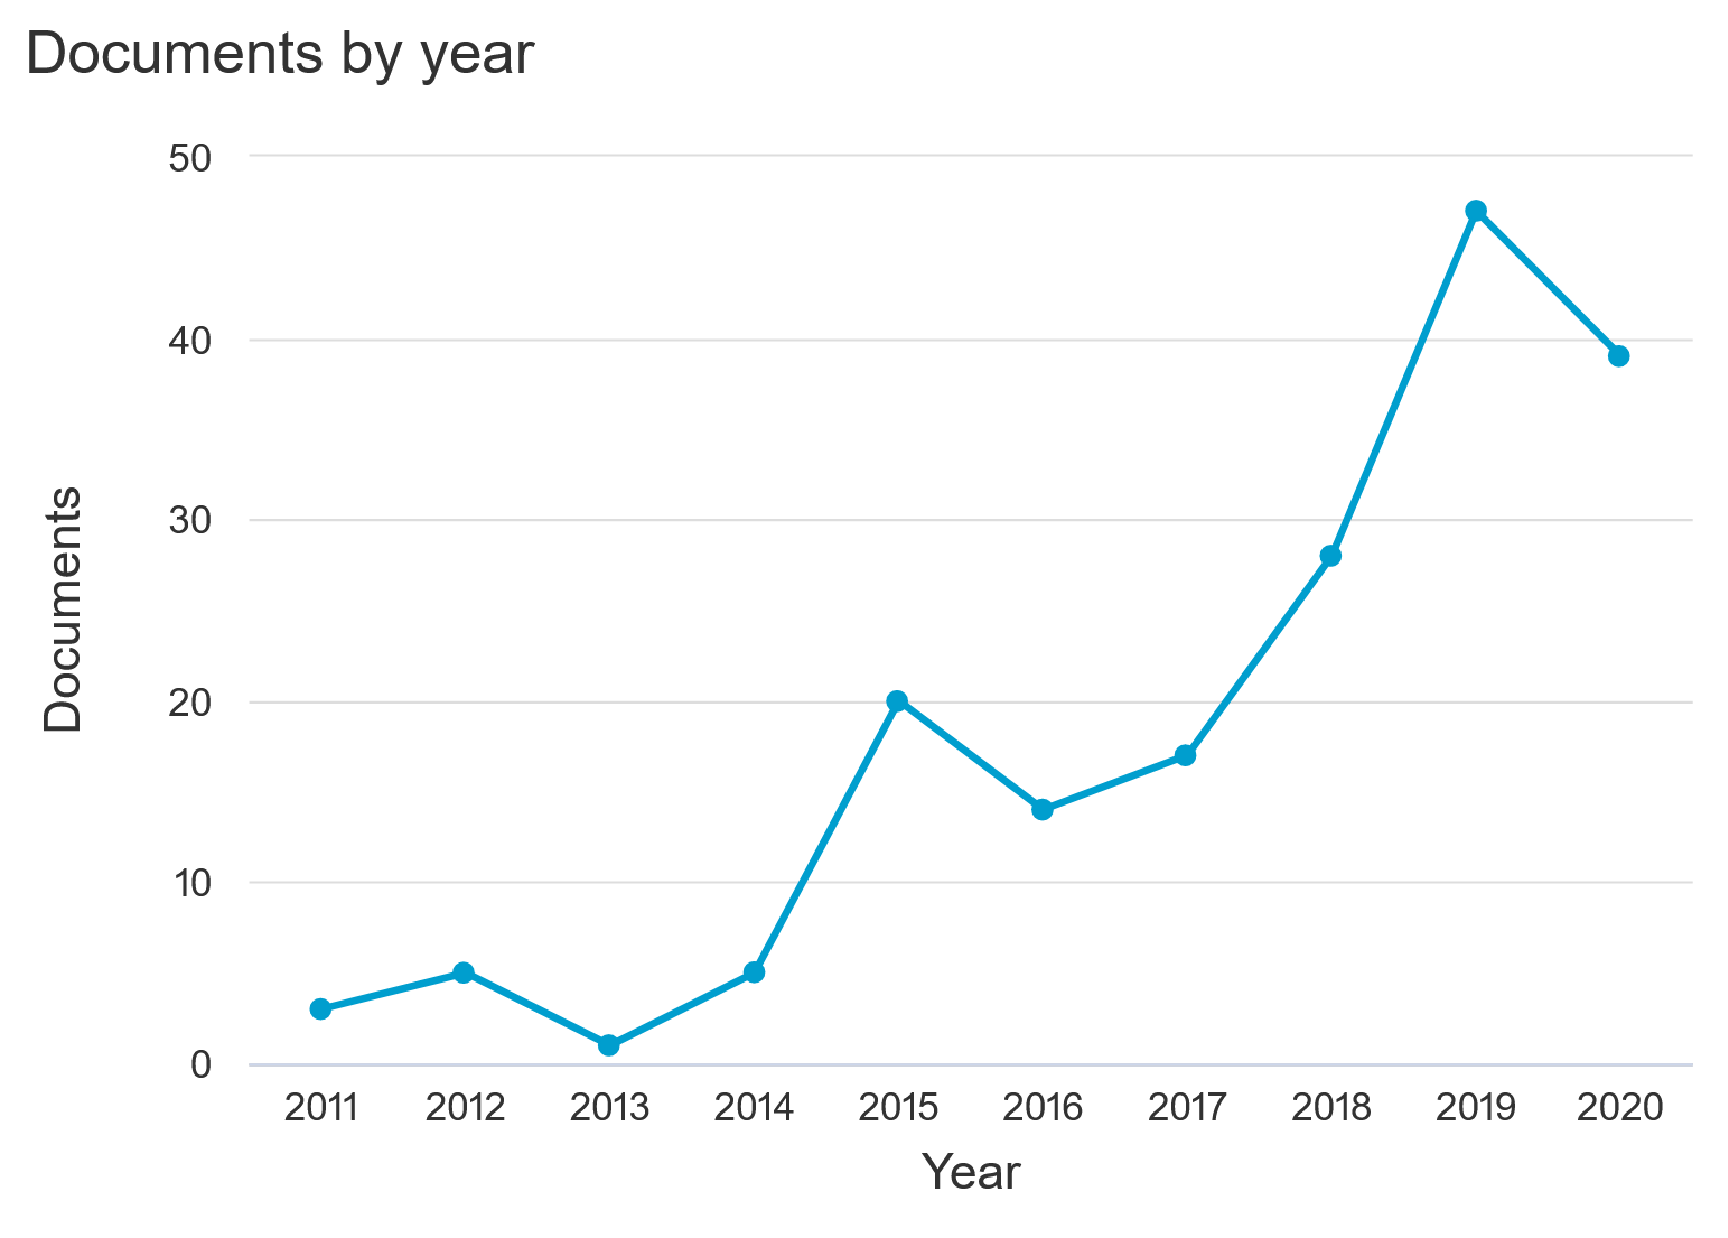
\includegraphics[width=\textwidth]{figures/chap-2/nlp-hist.pdf}
    \caption{Timelime of the volume of contributions per years for the crisis informatic domain. The year 2021 is excluded because the year is not complete at the time of writing.}
    \label{literature:nlp-hist}
\end{figure}

Figure~\ref{literature:nlp-bar}

\begin{figure}[bp]
    \centering
    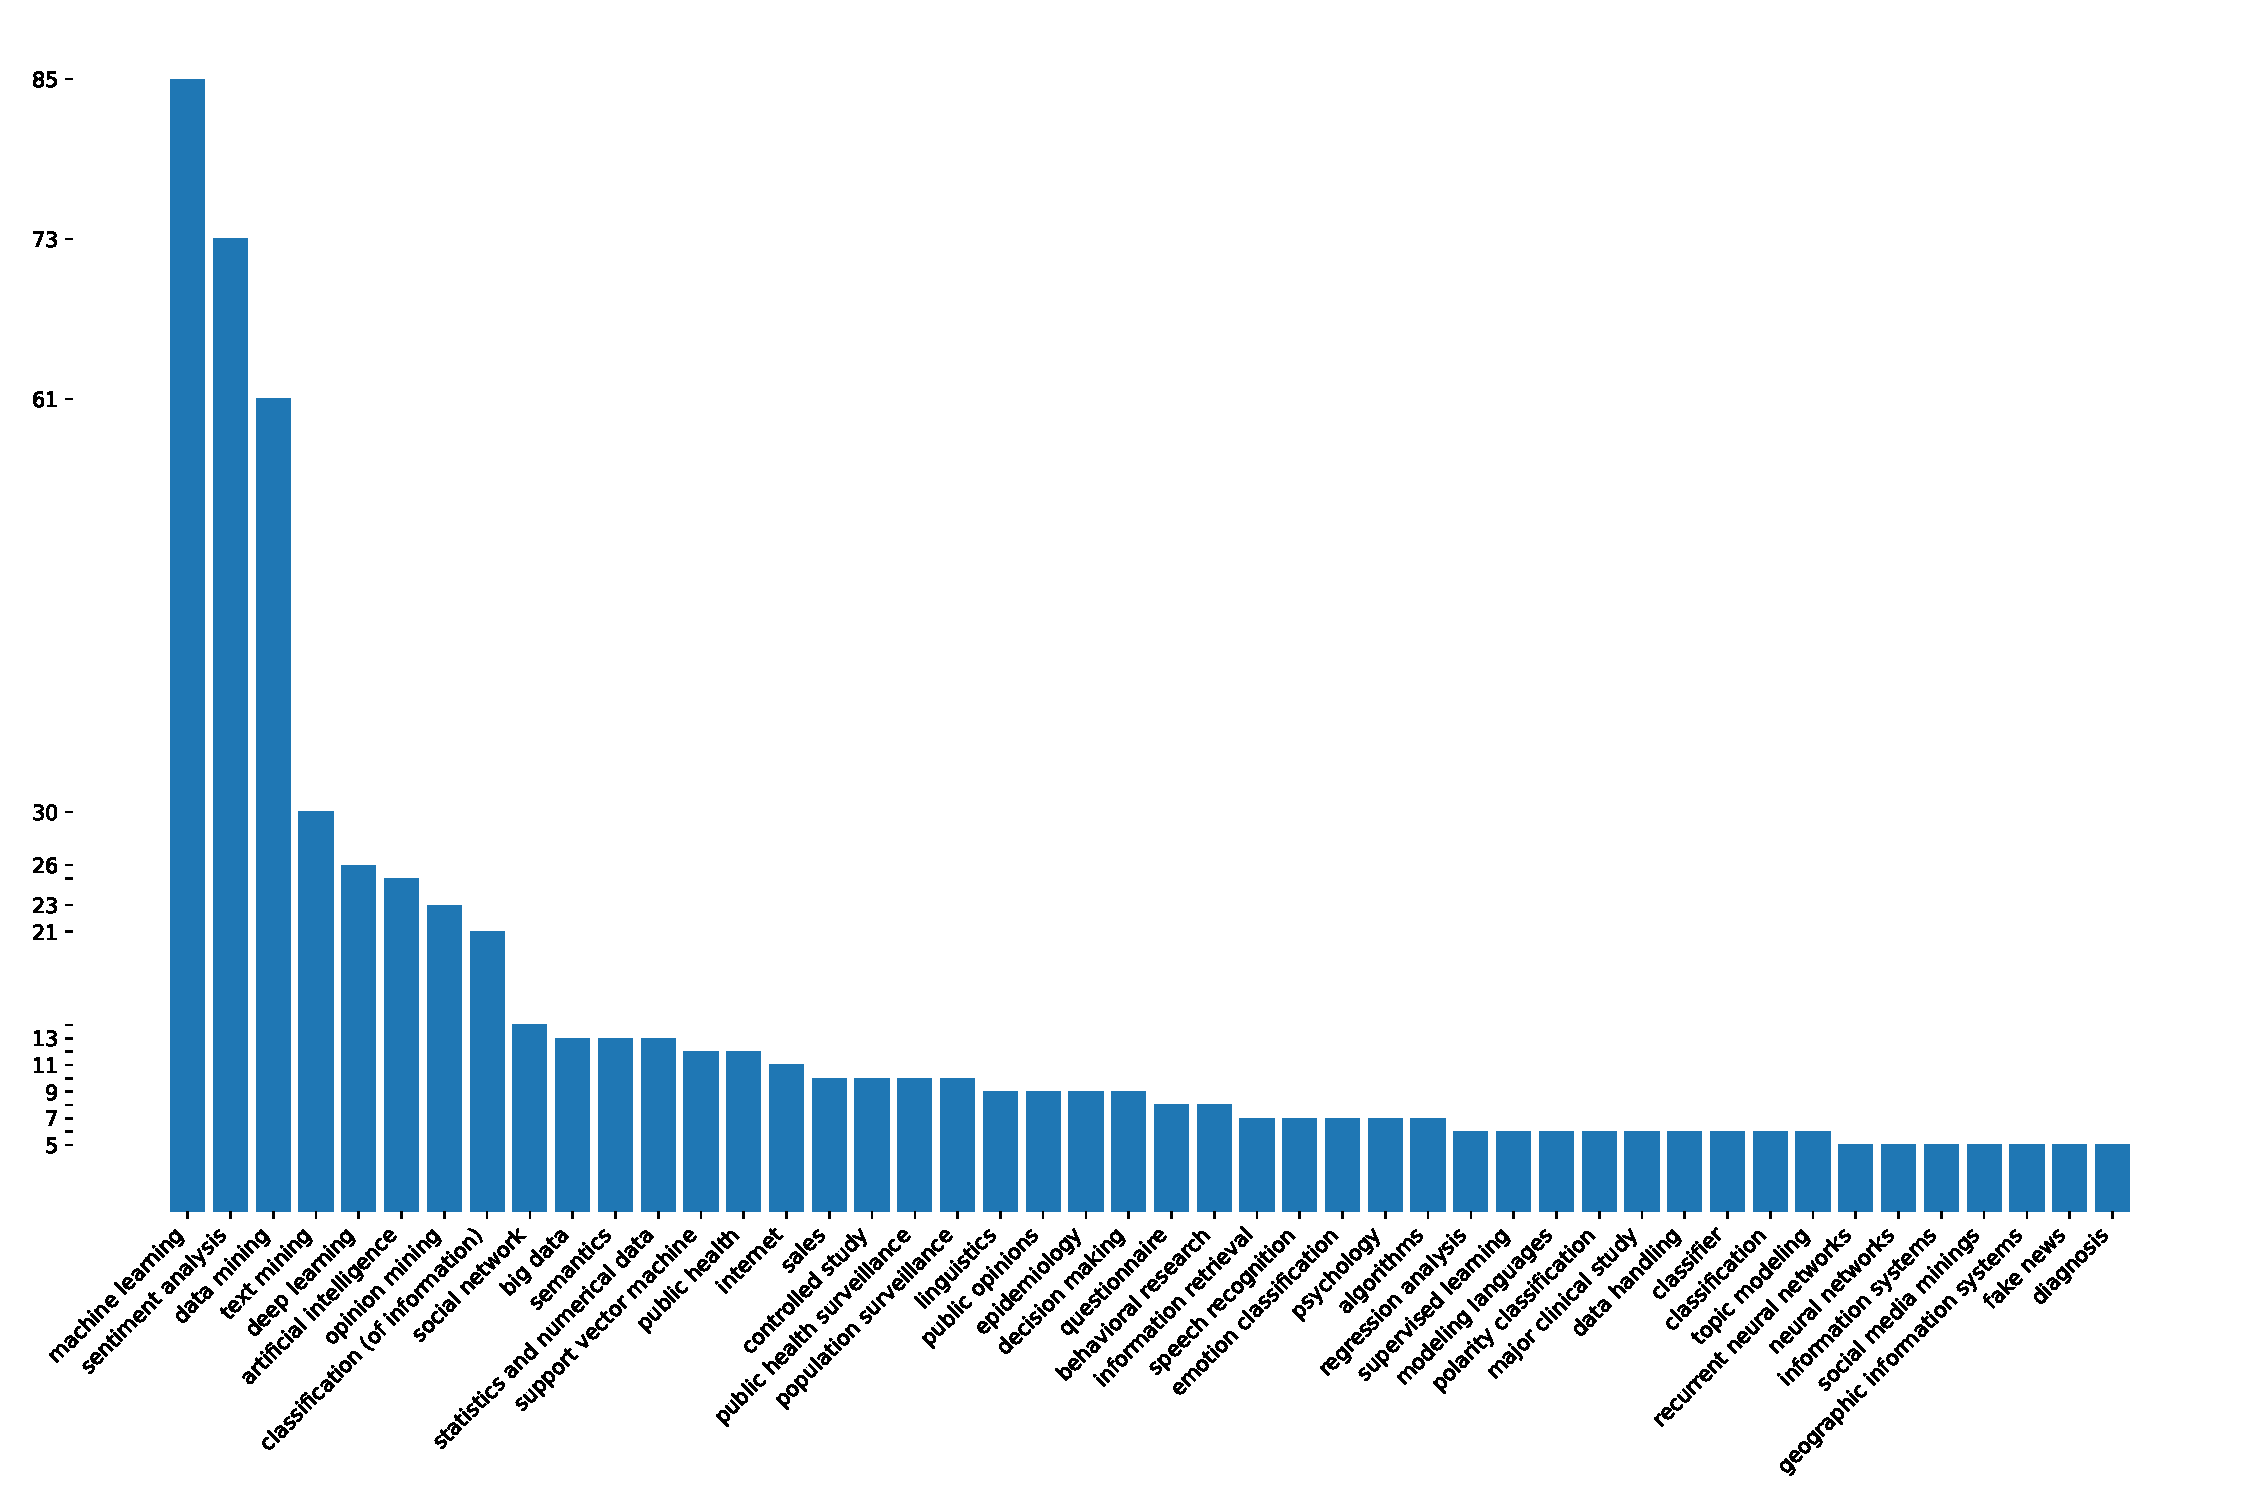
\includegraphics[width=\textwidth]{figures/chap-2/nlp-bar.pdf}
    \caption{Distribution of keywords with more than 3 occurrences among the articles from the query on crisis informatics. }
    \label{literature:nlp-bar}
\end{figure}

Figure~\ref{literature:nlp-overlay}

\begin{figure}[bp]
    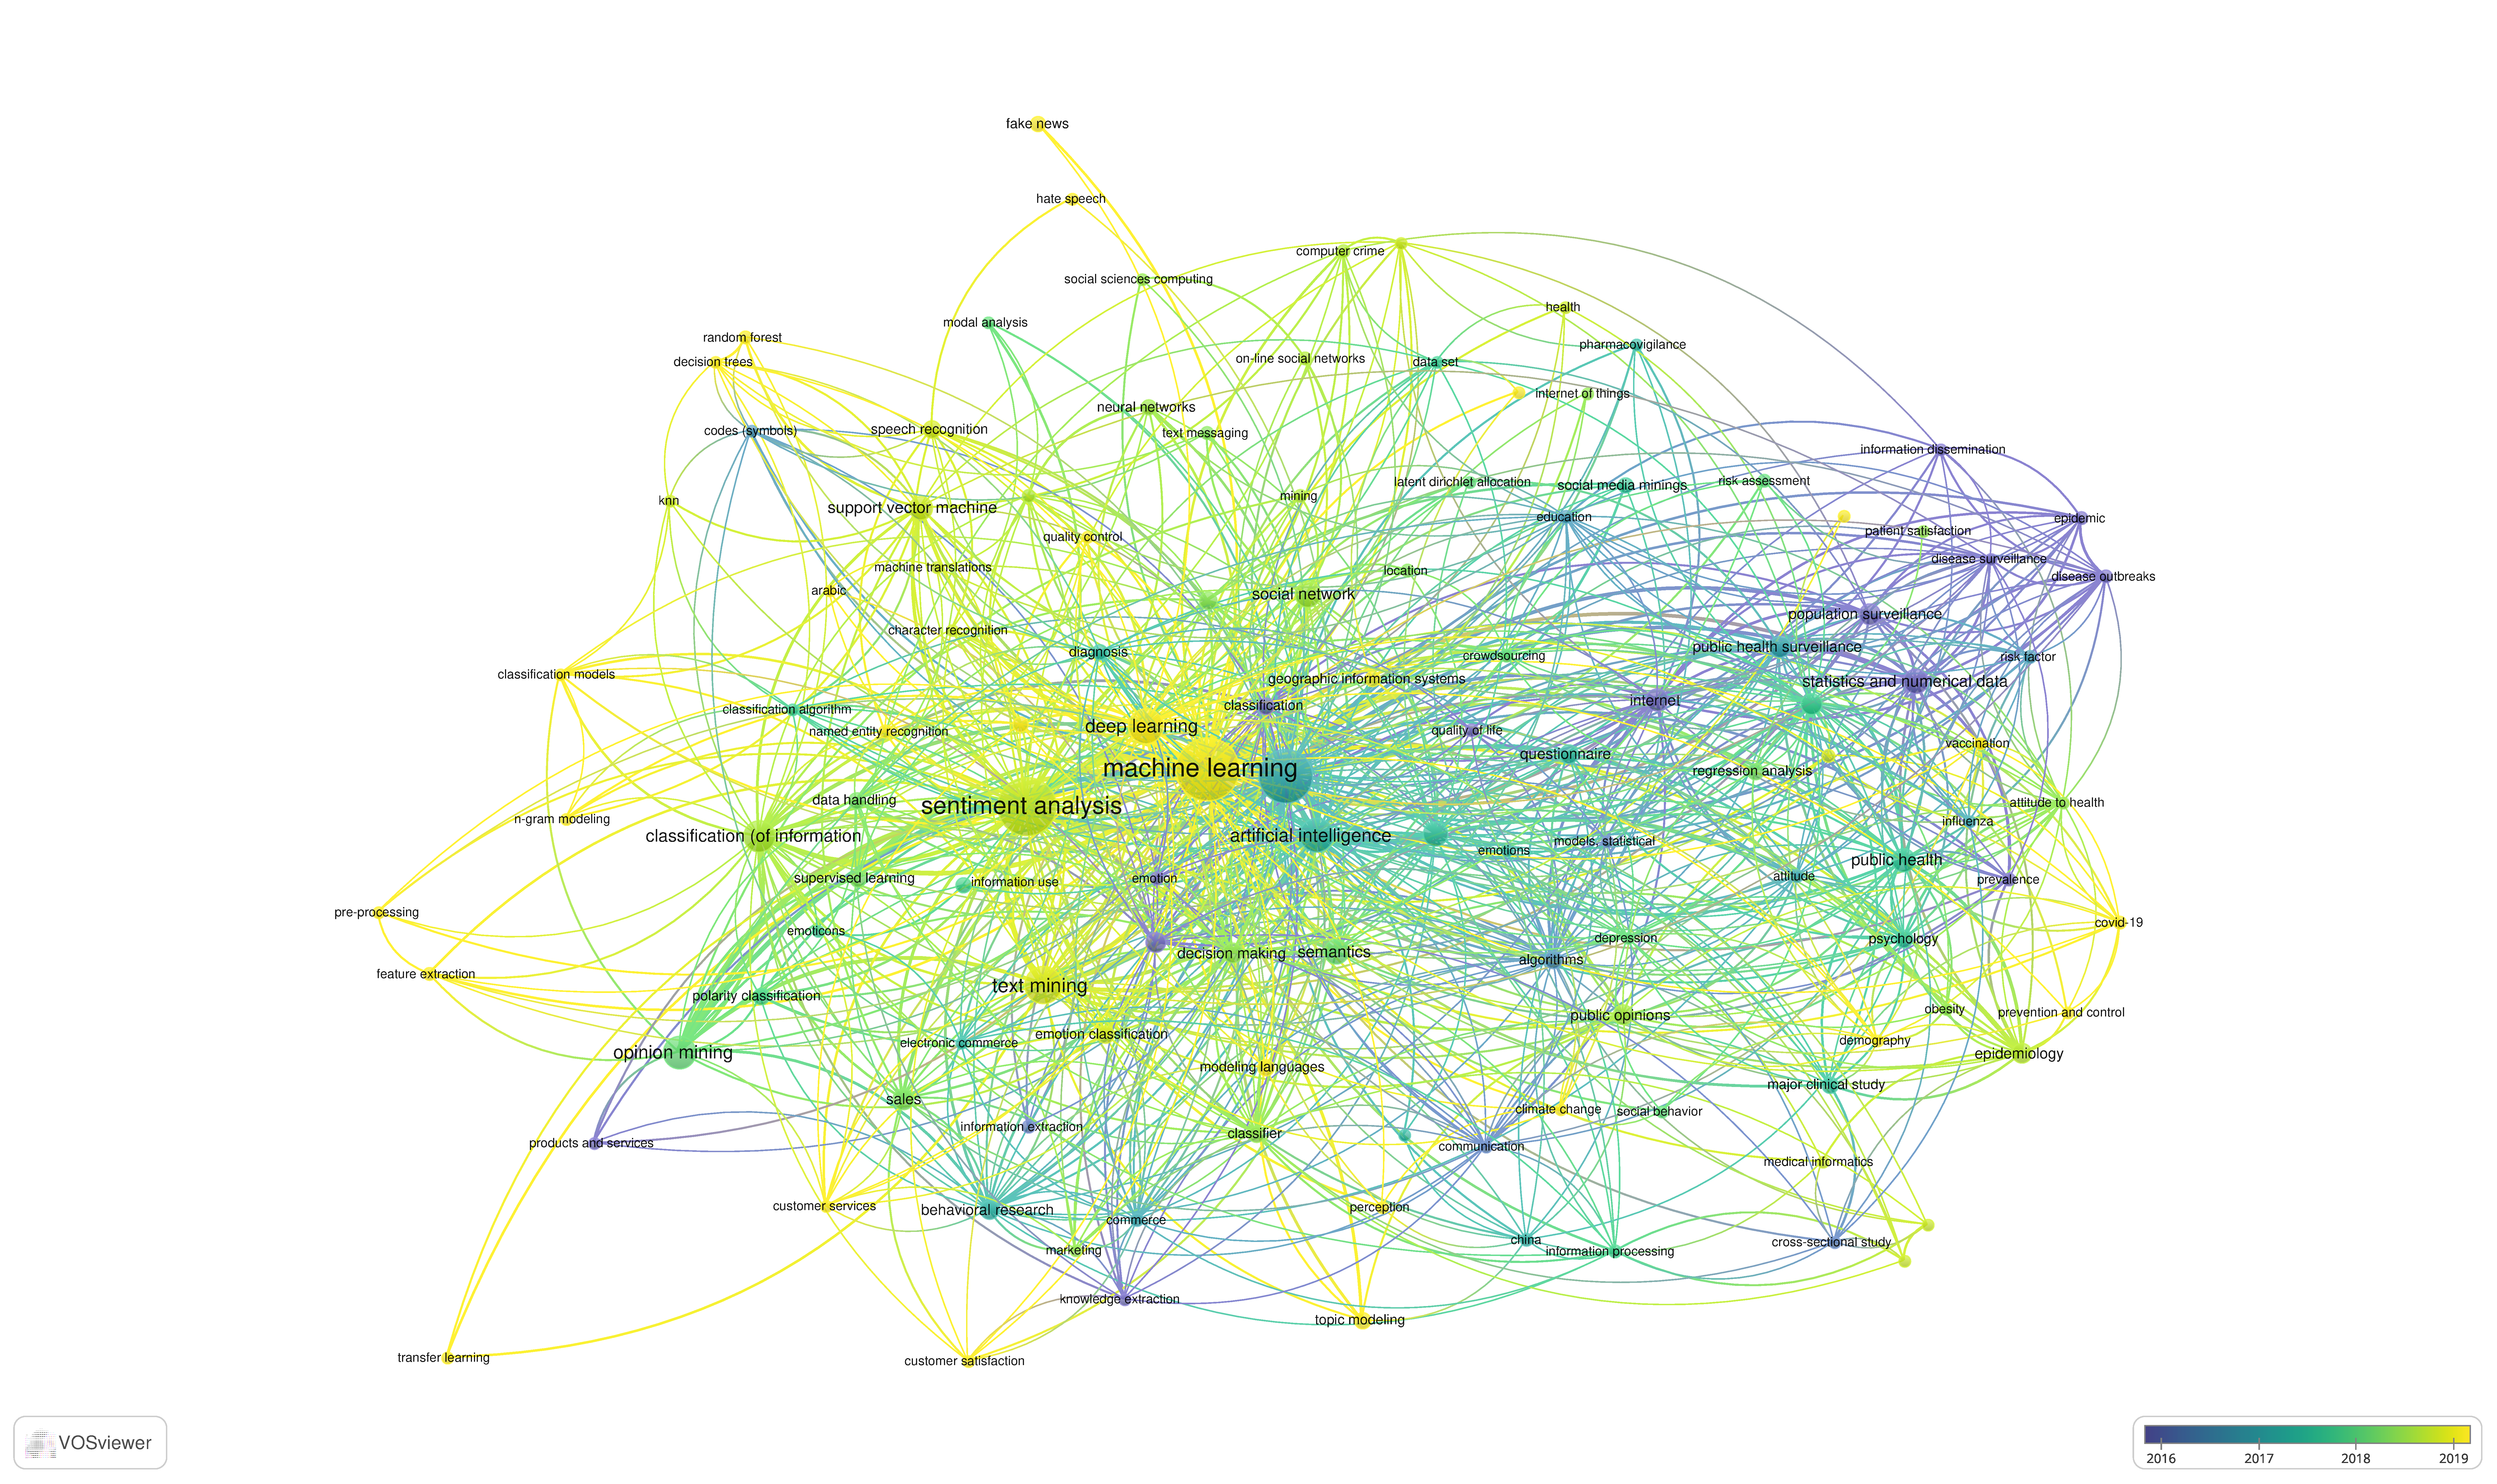
\includegraphics[width=\paperwidth,height=\paperheight,keepaspectratio, angle=90]{figures/chap-2/nlp-overlay.pdf}
    \caption{Distribution of keywords with more than 3 occurrences among the articles from the query on crisis informatics. }
    \label{literature:nlp-overlay}
\end{figure}



From the figure, it is possible to identify at least 2 clusters.
One cluster is oriented towards social and health sciences and applications of NLP on social media data in these domains.
The second one is more oriented towards computer sciences, specific algorithms and other applications domains.

Looking at the keywords that are common to at least 3 articles, we can identify several domains of application appear.
The keywords used by both the publishers and the authors also provide interesting insights.
Analyzing the keywords, three sets emerge:
\begin{itemize}
    \item Application domains: researchers identified areas of applications for NLP associated with social media data.
    \item Problem solving: general challenge of NLP translated to social media data or specific issue related to social media data.
    \item NLP techniques: the algorithms, approaches used to solve the previous challenges and relevant to an application domain.
\end{itemize}
For clarity, similar keywords (e.g. "emotions", "emotions analysis") are merged together in the tables for brevity.
The two following tables correspond to the two first sets (application domains and problem solving).
The next section dive deeper into the most common NLP techniques used.

Table~\ref{table:application-domains}

Many keywords where common to multiple topics. So instance "attitude" refers both to ...
"Quality of life" is used to urban issues, breast cancers, depression detection, opioids side effects.

\begin{center}
    \begin{longtable}{ rr }
        \hline
        Major domain          & Sub domains                     \\ [0.5ex]
        \hline
        Epidemiology          & COVID-19                        \\
                              & disease outbreaks               \\
                              & disease surveillance            \\
                              & vaccination                     \\
                              & epidemic                        \\
                              & epidemiology                    \\
                              & influenza                       \\
        \hline
        Medical Informatic    & depression                      \\
                              & diagnosis                       \\
                              & psychology                      \\
                              & public health surveillances     \\
                              & health survey                   \\
                              & risk factor                     \\
                              & major clinical study            \\
                              & medical informatics             \\
                              & obesity                         \\
                              & opiate addiction                \\
                              & opioid-related disorders        \\
                              & patient satisfaction            \\
                              & pharmacovigilance               \\
                              & pregnancy                       \\
                              & prevalence                      \\
                              & prevention and control          \\
                              & quality control                 \\
                              & risk assessment                 \\
                              & controlled study                \\
        \hline
        Behavioral Research   & social behavior                 \\
                              & models, statistical             \\
                              & social network                  \\
                              & computer crime                  \\
                              & public opinion                  \\
                              & population surveillance         \\
                              & demography                      \\
                              & smart city                      \\
                              & risk assessment                 \\
        \hline
        Social Media Research & facebook                        \\
                              & social media mining             \\
                              & fake news                       \\
                              & modal analysis                  \\
                              & data mining                     \\
                              & information dissemination       \\
                              & opinion mining                  \\
                              & perception                      \\
        \hline
        Business              & commerce                        \\
                              & customer services               \\
                              & sales                           \\
                              & communication                   \\
                              & electronic commerce             \\
                              & marketing                       \\
                              & products and services           \\
        \hline
        Information Science   & knowledge extraction            \\
                              & information systems             \\
                              & classification (of information) \\
                              & gis                             \\
                              & decision making                 \\
                              & information extraction          \\
                              & information processing          \\
        \hline
        NLP challenges        & machine translations            \\
                              & speech recognition              \\
                              & polarity classification         \\
                              & location inference              \\
                              & text mining                     \\
                              & automated detection             \\
                              & named entity recognition        \\
                              & arabic languages                \\
                              & linguistics                     \\
                              & topic modeling                  \\
                              & emotion analysis                \\
                              & sentiment analysis              \\
                              & emoticons                       \\
                              & modeling languages              \\
        \hline
        No specific category  & china                           \\
                              & education                       \\
                              & crowdsourcing                   \\
                              & climate change                  \\
                              & quality of life                 \\
                              & attitude                        \\
                              & internet of things              \\
                              & spatiotemporal analysis         \\
                              & surveys and questionnaires      \\
        \hline
        \caption{Applications domains}
        \label{table:application-domains}
    \end{longtable}
\end{center}

% Crisis informatic is not listed here – there are different definition of application domains
\cite{farzindarNaturalLanguageProcessing2017} identify several applications of NLP for social media data.
\begin{itemize}
    \item Geo-location detection
    \item Entity linking and Disambiguation
    \item Opinion mining and emotion analysis
    \item Event and topic detection
    \item Automatic summarization
    \item Machine translation
\end{itemize}

\subsection{NLP's tools to process previous data}

Along with this list of application, we can add the list of NLP techniques listed alongside:
\begin{table}[bp]
    \centering
    \begin{tabular}{rr}
        Major category          & Sub category                 \\ [0.5ex]
        \toprule
        Data management         & Big Data                     \\
                                & Pre-processing               \\
                                & N-gram Modeling              \\
        Artificial intelligence & Artificial Intelligence      \\
                                & Algorithms                   \\
                                & Classification Algorithms    \\
                                & Regression Analysis          \\
                                & Statistical Model            \\
                                & K-Nearest Neighbors          \\
        Machine learning        & Classifiers                  \\
                                & Supervised Learning          \\
                                & Feature Extraction           \\
                                & Decision Trees               \\
                                & Random Forests               \\
                                & Latent Dirichlet Allocation  \\
                                & Support Vector Machine       \\
        Deep learning           & Neural Networks              \\
                                & Classification Models        \\
                                & Transfer Learning            \\
                                & Convolutional Neural Network \\
                                & Recurrent Neural Networks    \\
        \bottomrule
    \end{tabular}
    \caption{Main NLP algorithms and techniques that appear among the keywords}
    \label{table:nlp-tools}
\end{table}

% Faire une partie qui décrit chaque point et les articles associés.
% Conclusion: le traitement des médias sociaux à très largement profité des avancées successives en intelligence artificelles qui ont été appliqués au NLP.
% Cette tendance s'observe temporellement, avec un léger décalage entre le moment ou l'algorithme/la techique devient mainstream et son adoption.

% \subsection{Processing of whole messages in social media data}
% - Informations à l'échelle du message complet (métadonnées + texte)
% - Informations à l'échelle du message textuel
% - Informations à l'échelle des mots du message.

% \begin{table}[bp]
%     \centering
%     \renewcommand{\arraystretch}{1.5}
%     \begin{tabular}{m{0.3\textwidth} m{0.7\textwidth}}
%         Reference                                             & Features \\ [0.5ex]
%         \toprule
%         \cite{liuSentimentAnalysisOpinion2012a}               &          \\
%         \cite{liuSurveyOpinionMining2012a}                    &          \\
%         \cite{collierUncoveringTextMining2012a}               &          \\
%         \cite{chamlertwatDiscoveringConsumerInsight2012a}     &          \\
%         \cite{bontchevaMakingSenseSocial2014a}                &          \\
%         \cite{vazquezClassificationUsergeneratedContent2014a} &          \\
%         \cite{raviSurveyOpinionMining2015a}                   &          \\
%         \cite{santillanaCombiningSearchSocial2015a}           &          \\
%         \cite{karmenScreeningInternetForum2015a}              &          \\
%         \cite{odlumWhatCanWe2015a}                            &          \\
%         \cite{linUncertaintyAnalysisCrowdsourced2015a}        &          \\
%         \cite{wangSocialMediaSensor2015a}                     &          \\
%         \cite{bahkPubliclyAvailableOnline2016a}               &          \\
%         \cite{paulSocialMediaMining2016a}                     &          \\
%         \cite{hawkinsMeasuringPatientperceivedQuality2016a}   &          \\
%         \cite{jiangAssessmentOnlinePublic2016a}               &          \\
%         \cite{bailCombiningNaturalLanguage2016a}              &          \\
%         \cite{kagasheEnhancingSeasonalInfluenza2017a}         &          \\
%         \cite{martinezPatientUnderstandingRisks2017a}         &          \\
%         \cite{poriaReviewAffectiveComputing2017a}             &          \\
%         \cite{yazdavarSemiSupervisedApproachMonitoring2017a}  &          \\
%         \cite{charyEpidemiologyTweetsEstimating2017a}         &          \\
%         \cite{salloumSurveyTextMining2017a}                   &          \\
%         \cite{sailunazEmotionDetectionText2018a}              &          \\
%         \cite{chaturvediDistinguishingFactsOpinions2018a}     &          \\
%         \cite{haririUncertaintyBigData2019a}                  &          \\
%         \cite{hemmatianSurveyClassificationTechniques2019a}   &          \\
%         \cite{yadavSentimentAnalysisUsing2020a}               &          \\
%         \bottomrule
%     \end{tabular}
%     \caption{Articles on informational needs of emergency responders retrieved from the previous request with at least 25 citations.}
%     \label{table:nlp-main-articles}
% \end{table}

%TODO Conclusion de la section  : qu'est-ce que finalement on peut exploiter comme information à partir des médias sociaux à l'aide du NLP

\section{Conclusions on the literature and identified gaps}
% Table with the business needs and the technical solution. Align both of them.
This section conclude the literature review and its outcome.
It takes the form of a table with two entries.
The first one is the identified informational needs of the decision makers.
The second one is the different technical solutions explored to extract information from social media data.
The contribution of this manuscript hold in the gap between these two domains.

1. Pas ou peu d'analyse du besoin des personnes qui utilisent les médias sociaux en situation de crise. Des classifications à l'arrache, parce qu'elle me plaît, parce que j'ai envie, parce que mon voisin à dit c'est cool.
-> Un modèle de situation de crise pour qui ? Pour quoi ?
2. Des tonnes d'architectures différentes, en fonction de comment le graduate a souhaité l'implémenter. Pas/peu de solution pour implémenter des données.
-> MLOps appliquées à notre problématique + mon architecture HICSS
3. Beaucoup de travaux pour classifier des messages. Peu de travaux sur le traitement à l'échelle du mot.


%%% Local Variables:
%%% mode: latex
%%% TeX-master: "../ma-these"
%%% End:
